\section{Bit of  Differential Geometry: Dayuum!!}
Let us look into a bit of differential geometry which is a formal way of treating this tensor thingy. We will try to be as intuitive and non-rigorous as possible (and thus increasing our chances of making a mathematician crazy!) but yeah, we will try to be rigorous enough so that I am satisfied.
\subsection{Some prior things}
Before touching manifolds, let us define what an abstract topological space is, since manifolds are special case of topological spaces. 
\begin{definition}[Topological Space]
  A topological space is a set $(X, \uptau )$ where $\uptau \subset \mathcal{P}$ is a collection of subsets of $X$ such that:
\begin{itemize}
    \item $\emptyset, X \in \uptau$.
    \item $U_\alpha \in \uptau \implies \bigcup \limits_{\alpha\in J} U_\alpha \in \uptau$  (closed under arbitrary union).
    \item $U_i \in \uptau \implies \bigcap \limits_{i=1}^n U_i \in \uptau$  (closed under finite intersection)\footnotemark.
\end{itemize}
\end{definition}
\footnote{Here $\alpha$ index is used when we want the indexing set $J$ (indexing set means the set from where the incides to denote the elements of the set are taken from) to be arbitrary, meaning that the set $\{U_\alpha\}$ can be finite, countable or uncountable. On the other hand, index $i$ is mostly used when the indexing set is finite.}

Well well, this does not look anything like coffee cup and donut which most people associate topology with. That is a case of \textit{homeomorphism} which will be discussed later (hopefully). However, for now let us proceed. The sets belonging to $\uptau$ are called \textbf{open sets}. We define a \textbf{closed set} as a set whose complement is open. There are umpteen other definitions like \textbf{closure, boundary, interior, neighbourhood}, etc. Let define few of them \emoji{loudly-crying-face}. 
\begin{itemize}
    \item \textit{Closure} of a set $A$ is the smallest closed set containing $A$ and is denoted by $\overline{A}$.
    \item \textit{Interior} of a set $A$ is the largest open set contained in $A$ and is denoted by $\text{int}(A)$.
    \item \textit{Boundary} of a set $A$ is the set of points which are neither in the interior nor in the exterior of $A$ and is denoted by $\partial A$.
    \item If $p\in X$, then a \textit{neighbourhood} of $p$ is a set $N$ such that there exists an open set $U\in \uptau$ with $p\in U\subseteq N$.
\begin{figure}[H]
      \centering
      

\tikzset{every picture/.style={line width=0.75pt}} %set default line width to 0.75pt        

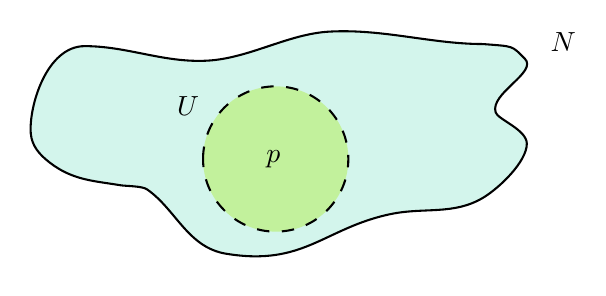
\begin{tikzpicture}[x=0.75pt,y=0.75pt,yscale=-1,xscale=1]
%uncomment if require: \path (0,203); %set diagram left start at 0, and has height of 203

%Curve Lines [id:da28281619681811754] 
\draw [fill={rgb, 255:red, 211; green, 245; blue, 236 }  ,fill opacity=1 ][line width=0.75] [line join = round][line cap = round]   (264,41.63) .. controls (239.07,41.63) and (216.02,34.24) .. (190,35.63) .. controls (169.94,36.71) and (151.25,48.57) .. (131,49.63) .. controls (109.98,50.74) and (92.57,42.63) .. (72,42.63) .. controls (53.59,42.63) and (45.01,71.73) .. (46,84.63) .. controls (46.47,90.7) and (50.18,94.88) .. (55,98.63) .. controls (66.08,107.25) and (76.24,107.51) .. (89,109.63) .. controls (91.95,110.13) and (99.58,109.96) .. (102,111.63) .. controls (115.88,121.24) and (121.56,139.56) .. (140,142.63) .. controls (177.55,148.89) and (187.14,130.46) .. (219,123.63) .. controls (235.52,120.09) and (249.69,124.22) .. (264,115.63) .. controls (271.71,111.01) and (285,98.32) .. (285,89.63) .. controls (285,82.9) and (271.1,77.94) .. (270,74.63) .. controls (266.91,65.36) and (290.59,55.22) .. (284,48.63) .. controls (277.54,42.17) and (279,42.85) .. (264,41.63) -- cycle ;
%Shape: Circle [id:dp001327175657310109] 
\draw  [fill={rgb, 255:red, 194; green, 241; blue, 156 }  ,fill opacity=1 ][dash pattern={on 4.5pt off 4.5pt}] (129,97) .. controls (129,77.67) and (144.67,62) .. (164,62) .. controls (183.33,62) and (199,77.67) .. (199,97) .. controls (199,116.33) and (183.33,132) .. (164,132) .. controls (144.67,132) and (129,116.33) .. (129,97) -- cycle ;

% Text Node
\draw (158,91.4) node [anchor=north west][inner sep=0.75pt]    {$p$};
% Text Node
\draw (115,65.4) node [anchor=north west][inner sep=0.75pt]    {$U$};
% Text Node
\draw (295,34.4) node [anchor=north west][inner sep=0.75pt]    {$N$};


\end{tikzpicture}

      \caption{Neighbourhood of a point $p$ in  $X$}
\end{figure}
          \item \textit{Hausdorff Space}: A topological space is called Hausdorff if for any two distinct points $x,y\in X$, there exist open sets $U,V\in \uptau$ such that $x\in U, y\in V$ and $U\cap V = \emptyset$. 
    \begin{figure}[H]
      \centering
      

\tikzset{every picture/.style={line width=0.75pt}} %set default line width to 0.75pt        

\begin{tikzpicture}[x=0.75pt,y=0.75pt,yscale=-1,xscale=1]
%uncomment if require: \path (0,203); %set diagram left start at 0, and has height of 203

%Shape: Circle [id:dp44753041237162206] 
\draw  [dash pattern={on 4.5pt off 4.5pt}] (129,97) .. controls (129,77.67) and (144.67,62) .. (164,62) .. controls (183.33,62) and (199,77.67) .. (199,97) .. controls (199,116.33) and (183.33,132) .. (164,132) .. controls (144.67,132) and (129,116.33) .. (129,97) -- cycle ;
%Shape: Circle [id:dp09577026242923825] 
\draw  [dash pattern={on 4.5pt off 4.5pt}] (230,98.5) .. controls (230,75.03) and (249.03,56) .. (272.5,56) .. controls (295.97,56) and (315,75.03) .. (315,98.5) .. controls (315,121.97) and (295.97,141) .. (272.5,141) .. controls (249.03,141) and (230,121.97) .. (230,98.5) -- cycle ;

% Text Node
\draw (159,92.4) node [anchor=north west][inner sep=0.75pt]    {$x$};
% Text Node
\draw (267,92.4) node [anchor=north west][inner sep=0.75pt]    {$y$};
% Text Node
\draw (113,56.4) node [anchor=north west][inner sep=0.75pt]    {$U$};
% Text Node
\draw (307,47.4) node [anchor=north west][inner sep=0.75pt]    {$V$};


\end{tikzpicture}

      \caption{A \textbf{Hausdorff Space}, where the points $x$ and $y$ are separated by the open sets $U$ and $V$.}
    \end{figure}
    \item \textit{Topological Continuity}: A function $f: X \to Y$ between two topological spaces is said to be continuous if for every open set $V \in \uptau_Y$, the preimage $f^{-1}(V)\footnote{The preimage of a set $Y$ under the function $f$ is defined as $f^{-1}(Y) = \{x|f(x)\in Y\}$. Note that this has nothing to do with inverse of a function (sadly we use the same notation)} \in \uptau_X$ is open in $X$.
    \item \textit{Homeomorphism}: A homeomorphism is a bijective function $f: X\to Y$ between two topological spaces such that both $f$ and its inverse $f^{-1}$ are continuous. If such a function exists, we say that the two spaces are \textbf{homeomorphic} and we write $X\cong Y$.
    \item \textit{Cover:} A cover of a topological space $X$ is a collection of sets $\{U_\alpha \}$whose union is $X$ that is, $\bigcup\limits_\alpha U_\alpha = X$. If each set is an open set, then it is called an \textbf{open cover}. If there exists a finite collection of subsets of the cover such that their union is $X$, that is, $\bigcup\limits_{i=1}^k U_i = X$ then it is called a \textbf{finite subcover}.
    \begin{figure}[H]
    \centering
    

\tikzset{every picture/.style={line width=0.75pt}} %set default line width to 0.75pt        

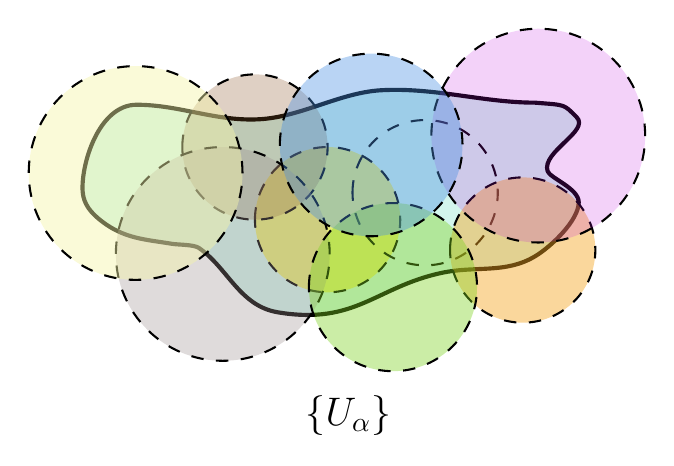
\begin{tikzpicture}[x=0.75pt,y=0.75pt,yscale=-1,xscale=1]
%uncomment if require: \path (0,227); %set diagram left start at 0, and has height of 227

%Curve Lines [id:da28281619681811754] 
\draw [fill={rgb, 255:red, 211; green, 245; blue, 236 }  ,fill opacity=1 ][line width=1.5] [line join = round][line cap = round]   (264,40.63) .. controls (239.07,40.63) and (216.02,33.24) .. (190,34.63) .. controls (169.94,35.71) and (151.25,47.57) .. (131,48.63) .. controls (109.98,49.74) and (92.57,41.63) .. (72,41.63) .. controls (53.59,41.63) and (45.01,70.73) .. (46,83.63) .. controls (46.47,89.7) and (50.18,93.88) .. (55,97.63) .. controls (66.08,106.25) and (76.24,106.51) .. (89,108.63) .. controls (91.95,109.13) and (99.58,108.96) .. (102,110.63) .. controls (115.88,120.24) and (121.56,138.56) .. (140,141.63) .. controls (177.55,147.89) and (187.14,129.46) .. (219,122.63) .. controls (235.52,119.09) and (249.69,123.22) .. (264,114.63) .. controls (271.71,110.01) and (285,97.32) .. (285,88.63) .. controls (285,81.9) and (271.1,76.94) .. (270,73.63) .. controls (266.91,64.36) and (290.59,54.22) .. (284,47.63) .. controls (277.54,41.17) and (279,41.85) .. (264,40.63) -- cycle ;
%Shape: Circle [id:dp001327175657310109] 
\draw  [fill={rgb, 255:red, 248; green, 231; blue, 28 }  ,fill opacity=0.55 ][dash pattern={on 4.5pt off 4.5pt}] (129,97) .. controls (129,77.67) and (144.67,62) .. (164,62) .. controls (183.33,62) and (199,77.67) .. (199,97) .. controls (199,116.33) and (183.33,132) .. (164,132) .. controls (144.67,132) and (129,116.33) .. (129,97) -- cycle ;
%Shape: Circle [id:dp7871419017635473] 
\draw  [dash pattern={on 4.5pt off 4.5pt}] (176,84) .. controls (176,64.67) and (191.67,49) .. (211,49) .. controls (230.33,49) and (246,64.67) .. (246,84) .. controls (246,103.33) and (230.33,119) .. (211,119) .. controls (191.67,119) and (176,103.33) .. (176,84) -- cycle ;
%Shape: Circle [id:dp8717686595013016] 
\draw  [fill={rgb, 255:red, 245; green, 166; blue, 35 }  ,fill opacity=0.45 ][dash pattern={on 4.5pt off 4.5pt}] (223,111.63) .. controls (223,92.3) and (238.67,76.63) .. (258,76.63) .. controls (277.33,76.63) and (293,92.3) .. (293,111.63) .. controls (293,130.96) and (277.33,146.63) .. (258,146.63) .. controls (238.67,146.63) and (223,130.96) .. (223,111.63) -- cycle ;
%Shape: Circle [id:dp9588061758851951] 
\draw  [fill={rgb, 255:red, 139; green, 87; blue, 42 }  ,fill opacity=0.28 ][dash pattern={on 4.5pt off 4.5pt}] (94,62) .. controls (94,42.67) and (109.67,27) .. (129,27) .. controls (148.33,27) and (164,42.67) .. (164,62) .. controls (164,81.33) and (148.33,97) .. (129,97) .. controls (109.67,97) and (94,81.33) .. (94,62) -- cycle ;
%Shape: Circle [id:dp9449595488988661] 
\draw  [fill={rgb, 255:red, 158; green, 145; blue, 145 }  ,fill opacity=0.33 ][dash pattern={on 4.5pt off 4.5pt}] (62,113.5) .. controls (62,85.06) and (85.06,62) .. (113.5,62) .. controls (141.94,62) and (165,85.06) .. (165,113.5) .. controls (165,141.94) and (141.94,165) .. (113.5,165) .. controls (85.06,165) and (62,141.94) .. (62,113.5) -- cycle ;
%Shape: Circle [id:dp5330131974534975] 
\draw  [fill={rgb, 255:red, 189; green, 16; blue, 224 }  ,fill opacity=0.19 ][dash pattern={on 4.5pt off 4.5pt}] (214,56.5) .. controls (214,28.06) and (237.06,5) .. (265.5,5) .. controls (293.94,5) and (317,28.06) .. (317,56.5) .. controls (317,84.94) and (293.94,108) .. (265.5,108) .. controls (237.06,108) and (214,84.94) .. (214,56.5) -- cycle ;
%Shape: Circle [id:dp4837000860245192] 
\draw  [fill={rgb, 255:red, 126; green, 211; blue, 33 }  ,fill opacity=0.4 ][dash pattern={on 4.5pt off 4.5pt}] (155,129.5) .. controls (155,107.13) and (173.13,89) .. (195.5,89) .. controls (217.87,89) and (236,107.13) .. (236,129.5) .. controls (236,151.87) and (217.87,170) .. (195.5,170) .. controls (173.13,170) and (155,151.87) .. (155,129.5) -- cycle ;
%Shape: Circle [id:dp17768072579265115] 
\draw  [fill={rgb, 255:red, 74; green, 144; blue, 226 }  ,fill opacity=0.39 ][dash pattern={on 4.5pt off 4.5pt}] (141,61) .. controls (141,36.7) and (160.7,17) .. (185,17) .. controls (209.3,17) and (229,36.7) .. (229,61) .. controls (229,85.3) and (209.3,105) .. (185,105) .. controls (160.7,105) and (141,85.3) .. (141,61) -- cycle ;
%Shape: Circle [id:dp406181221930618] 
\draw  [fill={rgb, 255:red, 244; green, 245; blue, 168 }  ,fill opacity=0.45 ][dash pattern={on 4.5pt off 4.5pt}] (20,74.5) .. controls (20,46.06) and (43.06,23) .. (71.5,23) .. controls (99.94,23) and (123,46.06) .. (123,74.5) .. controls (123,102.94) and (99.94,126) .. (71.5,126) .. controls (43.06,126) and (20,102.94) .. (20,74.5) -- cycle ;

% Text Node
\draw (152,180.4) node [anchor=north west][inner sep=0.75pt]  [font=\Large]  {$\{U_{\alpha }\}$};


\end{tikzpicture}

    \caption{Open cover of a space}
  \end{figure}
  \item \textit{Subspace Topology }is the topology on a subset $Y\subseteq X$ induced by the topology of $X$. In this case, open sets of $Y$ are basically the intersection of open sets of $X$ with $Y$. So,
  $$\uptau_Y = \{U\cap Y| U\in \uptau_X\}$$
  \end{itemize}
\subsection{Manifolds}
Let us see some pictures. 
\begin{figure}[H]
  \centering

  \begin{subfigure}[b]{0.3\textwidth}
    \centering
    

\tikzset{every picture/.style={line width=0.75pt}} %set default line width to 0.75pt        

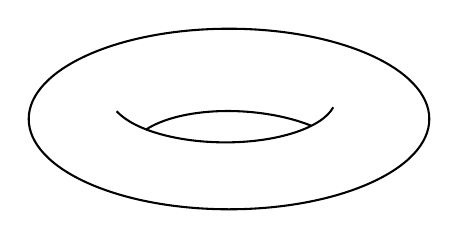
\begin{tikzpicture}[x=0.75pt,y=0.75pt,yscale=-1,xscale=1]
%uncomment if require: \path (0,300); %set diagram left start at 0, and has height of 300

%Shape: Ellipse [id:dp22801969143067424] 
\draw   (104,164.5) .. controls (104,140.48) and (147.2,121) .. (200.5,121) .. controls (253.8,121) and (297,140.48) .. (297,164.5) .. controls (297,188.52) and (253.8,208) .. (200.5,208) .. controls (147.2,208) and (104,188.52) .. (104,164.5) -- cycle ;
%Shape: Arc [id:dp10077529814620967] 
\draw  [draw opacity=0] (250.72,158.87) .. controls (245.28,168.82) and (223.36,176.06) .. (197.24,175.75) .. controls (173.88,175.48) and (154.02,169.25) .. (146.36,160.73) -- (197.5,153.5) -- cycle ; \draw   (250.72,158.87) .. controls (245.28,168.82) and (223.36,176.06) .. (197.24,175.75) .. controls (173.88,175.48) and (154.02,169.25) .. (146.36,160.73) ;  
%Shape: Arc [id:dp345385029103655] 
\draw  [draw opacity=0] (160.45,169.6) .. controls (170.37,163.16) and (188.19,159.59) .. (208.22,160.93) .. controls (220.26,161.74) and (231.27,164.2) .. (240.09,167.72) -- (206.61,184.82) -- cycle ; \draw   (160.45,169.6) .. controls (170.37,163.16) and (188.19,159.59) .. (208.22,160.93) .. controls (220.26,161.74) and (231.27,164.2) .. (240.09,167.72) ;  





\end{tikzpicture}

    \caption{Torus (yeah, donut came atlast!)}
  \end{subfigure}
  \hfill
  \begin{subfigure}[b]{0.3\textwidth}
    \centering
    

\tikzset{every picture/.style={line width=0.75pt}} %set default line width to 0.75pt        

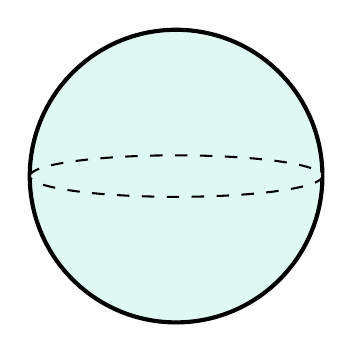
\begin{tikzpicture}[x=0.75pt,y=0.75pt,yscale=-1,xscale=1]
%uncomment if require: \path (0,300); %set diagram left start at 0, and has height of 300

%Shape: Circle [id:dp5828809729635696] 
\draw  [fill={rgb, 255:red, 223; green, 248; blue, 241 }  ,fill opacity=1 ][line width=1.5]  (161,152.5) .. controls (161,113.56) and (192.56,82) .. (231.5,82) .. controls (270.44,82) and (302,113.56) .. (302,152.5) .. controls (302,191.44) and (270.44,223) .. (231.5,223) .. controls (192.56,223) and (161,191.44) .. (161,152.5) -- cycle ;
%Shape: Ellipse [id:dp9903216585683989] 
\draw  [fill={rgb, 255:red, 223; green, 248; blue, 241 }  ,fill opacity=1 ][dash pattern={on 4.5pt off 4.5pt}] (161,152.5) .. controls (161,146.98) and (192.56,142.5) .. (231.5,142.5) .. controls (270.44,142.5) and (302,146.98) .. (302,152.5) .. controls (302,158.02) and (270.44,162.5) .. (231.5,162.5) .. controls (192.56,162.5) and (161,158.02) .. (161,152.5) -- cycle ;




\end{tikzpicture}

    \caption{Sphere (like yo mama)}
  \end{subfigure}
  \hfill
  \begin{subfigure}[b]{0.3\textwidth}
    \centering
    

\tikzset{every picture/.style={line width=0.75pt}} %set default line width to 0.75pt        

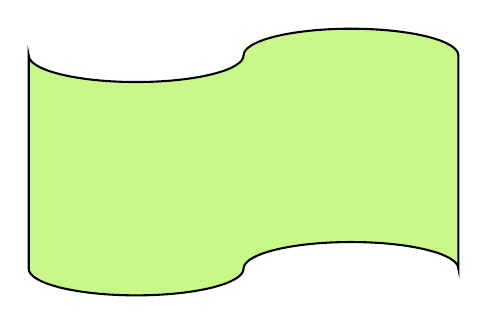
\begin{tikzpicture}[x=0.75pt,y=0.75pt,yscale=-1,xscale=1]
%uncomment if require: \path (0,300); %set diagram left start at 0, and has height of 300

%Flowchart: Punched Tape [id:dp25700721970086793] 
\draw  [fill={rgb, 255:red, 201; green, 248; blue, 137 }  ,fill opacity=1 ] (155,67.85) .. controls (155,74.94) and (178.17,80.69) .. (206.75,80.69) .. controls (235.33,80.69) and (258.5,74.94) .. (258.5,67.85) .. controls (258.5,60.75) and (281.67,55) .. (310.25,55) .. controls (338.83,55) and (362,60.75) .. (362,67.85) -- (362,170.62) .. controls (362,163.52) and (338.83,157.77) .. (310.25,157.77) .. controls (281.67,157.77) and (258.5,163.52) .. (258.5,170.62) .. controls (258.5,177.72) and (235.33,183.47) .. (206.75,183.47) .. controls (178.17,183.47) and (155,177.72) .. (155,170.62) -- cycle ;




\end{tikzpicture}

    \caption{A Waving Flag perhaps?}
  \end{subfigure}

  \caption{\textbf{What's common in all these?}}
\end{figure}
\noindent
So, what is common in all these pictures? Note that they all look very different from each other but if we really ZOOM in \emoji{mag-right} we can see that each of them look alike, like a \textit{flat plane}. Well, the road ahead of us looks flat but the road is on the freaking Earth which is, let's say to a physicist's satisfaction, a sphere. So, we can say that all of these things look `locally' like the flat plane $\mathbb{R}^2$. This is essentially the idea behind a \textbf{manifold}, things which look locally Euclidean (like $\mathbb{R}^n$). Let us define manifolds formally:
\begin{definition}[Differentiable Manifold]
  $\mathcal{M}$ is a m-dimensional differentiable manifold if:
  \begin{itemize}
    \item $\mathcal{M}$ is a topological space.
    \item There exists an open cover $\{U_\alpha\}$ of $\mathcal{M}$ and for each $\alpha$, there exists a homeomorphism $\phi_\alpha: U_\alpha \to V_\alpha$ where $V_\alpha$ is an open subset of $\mathbb{R}^m$.
    \item Two open sets $U_i, U_j$ such that $U_i \cap U_j \neq \emptyset$, then the map $\psi_{ij} = \phi_i \circ \phi_j^{-1}$ is a smooth map \footnotemark, where $\psi_{ij}: \phi_j(U_i \cap U_j) \to \phi_i(U_i \cap U_j)$.
  \end{itemize}
\end{definition}
\footnotetext{
A smooth map is a function which is infinitely differentiable, that is, all the derivatives exist and are continuous. Sometimes a smooth map $f$ is said to belong to the class $C^\infty$. In general, $C^k$ is the class of functions which are $k$ times continuously differentiable. \textcolor{blue}{We will consider mostly `smooth' things here, so we will always in general take $k$ to be $\infty$}}
\begin{figure}[H]
  \centering 
  

% Pattern Info
 
\tikzset{
pattern size/.store in=\mcSize, 
pattern size = 5pt,
pattern thickness/.store in=\mcThickness, 
pattern thickness = 0.3pt,
pattern radius/.store in=\mcRadius, 
pattern radius = 1pt}
\makeatletter
\pgfutil@ifundefined{pgf@pattern@name@_z2kbg8xsc}{
\pgfdeclarepatternformonly[\mcThickness,\mcSize]{_z2kbg8xsc}
{\pgfqpoint{0pt}{0pt}}
{\pgfpoint{\mcSize+\mcThickness}{\mcSize+\mcThickness}}
{\pgfpoint{\mcSize}{\mcSize}}
{
\pgfsetcolor{\tikz@pattern@color}
\pgfsetlinewidth{\mcThickness}
\pgfpathmoveto{\pgfqpoint{0pt}{0pt}}
\pgfpathlineto{\pgfpoint{\mcSize+\mcThickness}{\mcSize+\mcThickness}}
\pgfusepath{stroke}
}}
\makeatother

% Pattern Info
 
\tikzset{
pattern size/.store in=\mcSize, 
pattern size = 5pt,
pattern thickness/.store in=\mcThickness, 
pattern thickness = 0.3pt,
pattern radius/.store in=\mcRadius, 
pattern radius = 1pt}
\makeatletter
\pgfutil@ifundefined{pgf@pattern@name@_gl41bao2a}{
\pgfdeclarepatternformonly[\mcThickness,\mcSize]{_gl41bao2a}
{\pgfqpoint{0pt}{0pt}}
{\pgfpoint{\mcSize+\mcThickness}{\mcSize+\mcThickness}}
{\pgfpoint{\mcSize}{\mcSize}}
{
\pgfsetcolor{\tikz@pattern@color}
\pgfsetlinewidth{\mcThickness}
\pgfpathmoveto{\pgfqpoint{0pt}{0pt}}
\pgfpathlineto{\pgfpoint{\mcSize+\mcThickness}{\mcSize+\mcThickness}}
\pgfusepath{stroke}
}}
\makeatother

% Pattern Info
 
\tikzset{
pattern size/.store in=\mcSize, 
pattern size = 5pt,
pattern thickness/.store in=\mcThickness, 
pattern thickness = 0.3pt,
pattern radius/.store in=\mcRadius, 
pattern radius = 1pt}
\makeatletter
\pgfutil@ifundefined{pgf@pattern@name@_uzph2v4rp}{
\pgfdeclarepatternformonly[\mcThickness,\mcSize]{_uzph2v4rp}
{\pgfqpoint{0pt}{0pt}}
{\pgfpoint{\mcSize+\mcThickness}{\mcSize+\mcThickness}}
{\pgfpoint{\mcSize}{\mcSize}}
{
\pgfsetcolor{\tikz@pattern@color}
\pgfsetlinewidth{\mcThickness}
\pgfpathmoveto{\pgfqpoint{0pt}{0pt}}
\pgfpathlineto{\pgfpoint{\mcSize+\mcThickness}{\mcSize+\mcThickness}}
\pgfusepath{stroke}
}}
\makeatother
\tikzset{every picture/.style={line width=0.75pt}} %set default line width to 0.75pt        

\begin{tikzpicture}[x=0.75pt,y=0.75pt,yscale=-1,xscale=1]
%uncomment if require: \path (0,351); %set diagram left start at 0, and has height of 351

%Curve Lines [id:da574442534870605] 
\draw [fill={rgb, 255:red, 211; green, 245; blue, 236 }  ,fill opacity=1 ][line width=1.5] [line join = round][line cap = round]   (359,39.63) .. controls (334.07,39.63) and (311.02,32.24) .. (285,33.63) .. controls (264.94,34.71) and (246.25,46.57) .. (226,47.63) .. controls (204.98,48.74) and (187.57,40.63) .. (167,40.63) .. controls (148.59,40.63) and (140.01,69.73) .. (141,82.63) .. controls (141.47,88.7) and (145.18,92.88) .. (150,96.63) .. controls (161.08,105.25) and (171.24,105.51) .. (184,107.63) .. controls (186.95,108.13) and (194.58,107.96) .. (197,109.63) .. controls (210.88,119.24) and (216.56,137.56) .. (235,140.63) .. controls (272.55,146.89) and (282.14,128.46) .. (314,121.63) .. controls (330.52,118.09) and (344.69,122.22) .. (359,113.63) .. controls (366.71,109.01) and (380,96.32) .. (380,87.63) .. controls (380,80.9) and (366.1,75.94) .. (365,72.63) .. controls (361.91,63.36) and (385.59,53.22) .. (379,46.63) .. controls (372.54,40.17) and (374,40.85) .. (359,39.63) -- cycle ;
%Shape: Circle [id:dp6828648905721534] 
\draw  [fill={rgb, 255:red, 248; green, 231; blue, 28 }  ,fill opacity=0.55 ][dash pattern={on 4.5pt off 4.5pt}] (205,87) .. controls (205,67.67) and (220.67,52) .. (240,52) .. controls (259.33,52) and (275,67.67) .. (275,87) .. controls (275,106.33) and (259.33,122) .. (240,122) .. controls (220.67,122) and (205,106.33) .. (205,87) -- cycle ;
%Shape: Circle [id:dp30983551895185024] 
\draw  [fill={rgb, 255:red, 189; green, 16; blue, 224 }  ,fill opacity=0.19 ][dash pattern={on 4.5pt off 4.5pt}] (252,82.5) .. controls (252,60.68) and (269.68,43) .. (291.5,43) .. controls (313.32,43) and (331,60.68) .. (331,82.5) .. controls (331,104.32) and (313.32,122) .. (291.5,122) .. controls (269.68,122) and (252,104.32) .. (252,82.5) -- cycle ;
%Shape: Path Data [id:dp349889120130531] 
\draw  [pattern=_z2kbg8xsc,pattern size=6pt,pattern thickness=0.75pt,pattern radius=0pt, pattern color={rgb, 255:red, 0; green, 0; blue, 0}][dash pattern={on 4.5pt off 4.5pt}] (275,87) .. controls (275,96.62) and (271.12,105.33) .. (264.85,111.65) .. controls (256.95,104.43) and (252,94.04) .. (252,82.5) .. controls (252,73.43) and (255.06,65.08) .. (260.19,58.41) .. controls (269.15,64.75) and (275,75.19) .. (275,87) -- cycle ;
%Straight Lines [id:da4063749285607826] 
\draw    (225,108) -- (187.94,177.58) ;
\draw [shift={(187,179.35)}, rotate = 298.04] [color={rgb, 255:red, 0; green, 0; blue, 0 }  ][line width=0.75]    (10.93,-3.29) .. controls (6.95,-1.4) and (3.31,-0.3) .. (0,0) .. controls (3.31,0.3) and (6.95,1.4) .. (10.93,3.29)   ;
%Straight Lines [id:da2660552290852516] 
\draw    (303,98) -- (347.96,171.64) ;
\draw [shift={(349,173.35)}, rotate = 238.6] [color={rgb, 255:red, 0; green, 0; blue, 0 }  ][line width=0.75]    (10.93,-3.29) .. controls (6.95,-1.4) and (3.31,-0.3) .. (0,0) .. controls (3.31,0.3) and (6.95,1.4) .. (10.93,3.29)   ;
% Consistent, clean axis arrows using TikZ arrow tips
\draw[->, line width=1] (132,266) -- (232,266); % x-axis
\draw[->, line width=1] (142,276) -- (142,176); % y-axis

\draw[->, line width=1] (314,266) -- (414,266); % x-axis
\draw[->, line width=1] (324,273) -- (324,173); % y-axis
%Shape: Circle [id:dp3856434949934364] 
\draw  [fill={rgb, 255:red, 184; green, 233; blue, 134 }  ,fill opacity=0.63 ][dash pattern={on 4.5pt off 4.5pt}] (156,223.5) .. controls (156,210.52) and (166.52,200) .. (179.5,200) .. controls (192.48,200) and (203,210.52) .. (203,223.5) .. controls (203,236.48) and (192.48,247) .. (179.5,247) .. controls (166.52,247) and (156,236.48) .. (156,223.5) -- cycle ;
%Shape: Circle [id:dp6236997602250793] 
\draw  [fill={rgb, 255:red, 245; green, 166; blue, 35 }  ,fill opacity=0.57 ][dash pattern={on 4.5pt off 4.5pt}] (338,217.5) .. controls (338,199) and (353,184) .. (371.5,184) .. controls (390,184) and (405,199) .. (405,217.5) .. controls (405,236) and (390,251) .. (371.5,251) .. controls (353,251) and (338,236) .. (338,217.5) -- cycle ;
%Shape: Path Data [id:dp5971497523670923] 
\draw  [pattern=_gl41bao2a,pattern size=6pt,pattern thickness=0.75pt,pattern radius=0pt, pattern color={rgb, 255:red, 0; green, 0; blue, 0}][dash pattern={on 4.5pt off 4.5pt}] (203,223.71) .. controls (203,231.18) and (199.04,237.95) .. (192.62,242.87) .. controls (184.56,237.25) and (179.5,229.18) .. (179.5,220.21) .. controls (179.5,213.16) and (182.62,206.67) .. (187.87,201.48) .. controls (197.02,206.41) and (203,214.53) .. (203,223.71) -- cycle ;
%Shape: Path Data [id:dp038898347866279326] 
\draw  [pattern=_uzph2v4rp,pattern size=6pt,pattern thickness=0.75pt,pattern radius=0pt, pattern color={rgb, 255:red, 0; green, 0; blue, 0}][dash pattern={on 4.5pt off 4.5pt}] (363,221.67) .. controls (363,230.57) and (358.79,238.64) .. (351.96,244.49) .. controls (343.38,237.81) and (338,228.19) .. (338,217.5) .. controls (338,209.1) and (341.32,201.37) .. (346.91,195.19) .. controls (356.64,201.06) and (363,210.73) .. (363,221.67) -- cycle ;
%Straight Lines [id:da8518964920780053] 
\draw [line width=1.5]    (350,223.02) -- (194,224) ;
\draw [shift={(191,224.02)}, rotate = 359.64] [color={rgb, 255:red, 0; green, 0; blue, 0 }  ][line width=1.5]    (14.21,-4.28) .. controls (9.04,-1.82) and (4.3,-0.39) .. (0,0) .. controls (4.3,0.39) and (9.04,1.82) .. (14.21,4.28)   ;

% Text Node
\draw (181,66.4) node [anchor=north west][inner sep=0.75pt]    {$U_{i}$};
% Text Node
\draw (332,58.4) node [anchor=north west][inner sep=0.75pt]    {$U_{j}$};
% Text Node
\draw (175,280.4) node [anchor=north west][inner sep=0.75pt]    {$\mathbb{R}^{m}$};
% Text Node
\draw (359,280.4) node [anchor=north west][inner sep=0.75pt]    {$\mathbb{R}^{m}$};
% Text Node
\draw (199,188.4) node [anchor=north west][inner sep=0.75pt]    {$U_{i} '$};
% Text Node
\draw (404,190.4) node [anchor=north west][inner sep=0.75pt]    {$U_{j} '$};
% Text Node
\draw (180,131.4) node [anchor=north west][inner sep=0.75pt]    {$\phi _{i}$};
% Text Node
\draw (339,131.4) node [anchor=north west][inner sep=0.75pt]    {$\phi _{j}$};
% Text Node
\draw (257,195.4) node [anchor=north west][inner sep=0.75pt]  [font=\large]  {$\psi _{i}{}_{j}$};
% Text Node
\draw (396,32.4) node [anchor=north west][inner sep=0.75pt]  [font=\Large]  {$\mathcal{M}$};


\end{tikzpicture}

  \caption{The figure shows the third point in the definition. So basically, we note where the homeomorphisms map the intersection of the open sets and then define the map $\psi_{ij}$ between these two regions.}
\end{figure}
A point $p \in U \subset \mathcal{M}$ has the coordinates $(\phi^1(p),\ldots, \phi^m(p) )\in \mathbb{R}^m$ with respect to the chart $(U,\phi)$. The coordinate functions $\phi^i$ are defined in terms of the projection map $\mathrm{proj}_i:\mathbb{R}^m \longrightarrow \mathbb{R}$ such that $\mathrm{proj}_i(x) \mapsto x^i$\footnote{This just selects the $i^{\text{th}}$ component of a m-dimensional vector $x$ in $\mathbb{R}^m$} and $\phi^\mu: \mathcal{M}\rightarrow \mathbb{R}$ such that $p \mapsto \mathrm{proj}_\mu(\phi(p))$. So basically $\phi$ sends $p$ to some point in $\mathbb{R}^m$ and then to find the individual components, we take the projection of $\phi(p)$ along that coordinate. Henceforth we will use $r^i$ to denote $\mathrm{proj}_i$ (cause brevity is the soul of wit!) and also, to be familiar with our common sense, we will denote the coordinate maps $\phi^i$ with $x^i$, which actually gives us the feel of some coordinates.\\[0.3cm]
The terminologies used here are very much related to the geography of Earth. The pair $(U_i, \phi_i)$ is called a \textit{chart} (maybe because they help us to locally ``chart'' the manifold, that is, understand it using some coordinates) and the collection of all charts is called an \textit{atlas} (well, because it is collection of maps). \\[0.3cm]
Now let us unfold this carefully. For the open set $U_i$, the map $\phi_i$ takes it to another open set in $\mathbb{R}^m$. So for all $x\in U_i$ we got a mapping to an Euclidean space. Same goes for $U_j$, that is we obtain a mapping into another copy of $\mathbb{R}^m$. Now for points in the intersection of $U_i$ and $U_j$, we have got two different mappings and we can go back and forth between the two copies of $\mathbb{R}^m$ since these mappings were homeomorphisms. This is what we had with the mapping $\psi_{ij}$ (and thus, these are aptly called \textit{transition functions}). It first maps with the inverse of $\phi_j$  and then applies $\phi_i$. The net effect is that we are mapping between a point in one copy of $\mathbb{R}^m$ to another copy of $\mathbb{R}^m$. \\[0.3cm]
Imagine the open sets as patches in the manifold. We can then patch together the whole manifold by taking the union of all the open sets, all of which can be viewed as a Euclidean space. There are also manifolds which do not have the smooth property on the transient function, only continuity is there. These are called in general \textbf{topological manifolds}.\\[0.2cm]
] We also assume that our manifolds are \textbf{Hausdorff} and paracompact (which we will not define here). 
\begin{ffact}
For a differentiable manifold $\SM$, the set of smooth real-valued functions on it $C^\infty(\SM)$ is a \textit{ring}
\end{ffact}
\subsubsection{Examples:}
Now comes the good thing: examples! \emoji{smiling-face}
\textbf{The Space $\mathbf{\mathbb{R}^n}$}\\[0.3cm]
Duh, it looks like $\mathbb{R}^n$ locally since it is $\mathbb{R}^n$ itself. A single chart is enough for the purpose and the homeomorphism is the identity map. \\[0.3cm]
\textbf{The Circle $\mathbb{S}^1$}\\[0.3cm]
Circle is a curve in $\mathbb{R}^2$ with coordinates $(\cos\theta, \sin\theta)$. We mostly take $\theta \in [0,2\pi)$ but we come across a problem. Note that the open sets on a circle are basically union of ``open arcs''. However, $[0,2\pi)$ is not open. Thus we need atleast two charts to cover the circle.\\[0.3cm]
We take two antipodal points on the circle and then define the charts as follows: \\[0.3cm]
Let $U_1 = \mathbb{S}^1\backslash \{(1,0)\},U_2 = \mathbb{S}^1\backslash \{(-1,0)\}$. Then define the homeomorphisms as:
$$\phi_1: \mathbb{S}^1\backslash \{(1,0)\}\rightarrow (0,2\pi) \quad \quad \phi_2: \mathbb{S}^1\backslash \{(-1,0)\}\rightarrow (-\pi,\pi)$$
These functions basically take the value of the angle $\theta$ that a point on the circle makes with the x-axis.  
\begin{figure}[H]
  \centering
  \begin{subfigure}[b]{0.45\textwidth}
    \centering
    

\tikzset{every picture/.style={line width=0.75pt}} %set default line width to 0.75pt        

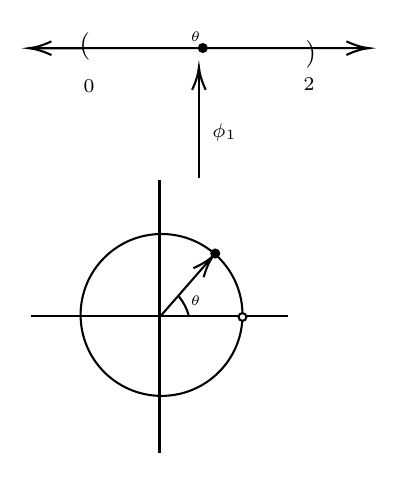
\begin{tikzpicture}[x=0.75pt,y=0.75pt,yscale=-1,xscale=1]
%uncomment if require: \path (0,300); %set diagram left start at 0, and has height of 300

\draw   (121,188.73) -- (245,188.73)(183,123) -- (183,254.47) ;
%Straight Lines [id:da8180273995647878] 
\draw    (122,59.5) -- (282,59.47) ;
\draw [shift={(284,59.47)}, rotate = 179.99] [color={rgb, 255:red, 0; green, 0; blue, 0 }  ][line width=0.75]    (10.93,-3.29) .. controls (6.95,-1.4) and (3.31,-0.3) .. (0,0) .. controls (3.31,0.3) and (6.95,1.4) .. (10.93,3.29)   ;
\draw [shift={(120,59.5)}, rotate = 359.99] [color={rgb, 255:red, 0; green, 0; blue, 0 }  ][line width=0.75]    (10.93,-3.29) .. controls (6.95,-1.4) and (3.31,-0.3) .. (0,0) .. controls (3.31,0.3) and (6.95,1.4) .. (10.93,3.29)   ;
%Shape: Circle [id:dp5128133772288312] 
\draw   (145,188) .. controls (145,166.46) and (162.46,149) .. (184,149) .. controls (205.54,149) and (223,166.46) .. (223,188) .. controls (223,209.54) and (205.54,227) .. (184,227) .. controls (162.46,227) and (145,209.54) .. (145,188) -- cycle ;
%Shape: Circle [id:dp8810895316002555] 
\draw  [fill={rgb, 255:red, 255; green, 255; blue, 255 }  ,fill opacity=1 ] (221.12,189) .. controls (221.12,187.96) and (221.96,187.12) .. (223,187.12) .. controls (224.04,187.12) and (224.88,187.96) .. (224.88,189) .. controls (224.88,190.04) and (224.04,190.88) .. (223,190.88) .. controls (221.96,190.88) and (221.12,190.04) .. (221.12,189) -- cycle ;
%Straight Lines [id:da9436577937186711] 
\draw    (184,188) -- (207.68,160.91) ;
\draw [shift={(209,159.4)}, rotate = 131.16] [color={rgb, 255:red, 0; green, 0; blue, 0 }  ][line width=0.75]    (10.93,-3.29) .. controls (6.95,-1.4) and (3.31,-0.3) .. (0,0) .. controls (3.31,0.3) and (6.95,1.4) .. (10.93,3.29)   ;
%Shape: Arc [id:dp6136432634457998] 
\draw  [draw opacity=0] (192.32,179.07) .. controls (194.56,181.78) and (196.24,184.99) .. (197.17,188.52) -- (174.15,194.94) -- cycle ; \draw   (192.32,179.07) .. controls (194.56,181.78) and (196.24,184.99) .. (197.17,188.52) ;  
%Straight Lines [id:da3473098561653878] 
\draw    (202,121.87) -- (202,70.62) ;
\draw [shift={(202,68.62)}, rotate = 90] [color={rgb, 255:red, 0; green, 0; blue, 0 }  ][line width=0.75]    (10.93,-3.29) .. controls (6.95,-1.4) and (3.31,-0.3) .. (0,0) .. controls (3.31,0.3) and (6.95,1.4) .. (10.93,3.29)   ;
%Shape: Circle [id:dp05894903245242711] 
\draw  [fill={rgb, 255:red, 0; green, 0; blue, 0 }  ,fill opacity=1 ] (208,158.4) .. controls (208,157.36) and (208.84,156.52) .. (209.88,156.52) .. controls (210.92,156.52) and (211.77,157.36) .. (211.77,158.4) .. controls (211.77,159.44) and (210.92,160.28) .. (209.88,160.28) .. controls (208.84,160.28) and (208,159.44) .. (208,158.4) -- cycle ;
%Shape: Circle [id:dp0797933236440207] 
\draw  [fill={rgb, 255:red, 0; green, 0; blue, 0 }  ,fill opacity=1 ] (202,59.4) .. controls (202,58.36) and (202.84,57.52) .. (203.88,57.52) .. controls (204.92,57.52) and (205.77,58.36) .. (205.77,59.4) .. controls (205.77,60.44) and (204.92,61.28) .. (203.88,61.28) .. controls (202.84,61.28) and (202,60.44) .. (202,59.4) -- cycle ;

% Text Node
\draw (196.5,177.1) node [anchor=north west][inner sep=0.75pt]  [font=\tiny]  {$\theta $};
% Text Node

% Text Node
\draw (142.88,50.5) node [anchor=north west][inner sep=0.75pt]  [rotate=-359.08]  {$($};
% Text Node
\draw (259.98,70.62) node [anchor=north west][inner sep=0.75pt]  [rotate=-180.17]  {$($};
% Text Node
\draw (144.88,73.5) node [anchor=north west][inner sep=0.75pt]  [font=\scriptsize,rotate=-359.08]  {$0$};
% Text Node
\draw (250.88,72.5) node [anchor=north west][inner sep=0.75pt]  [font=\scriptsize,rotate=-359.08]  {$2\uppi $};
% Text Node
\draw (196.5,50.1) node [anchor=north west][inner sep=0.75pt]  [font=\tiny]  {$\theta $};
% Text Node
\draw (206.88,94.5) node [anchor=north west][inner sep=0.75pt]  [font=\scriptsize,rotate=-359.08]  {$\phi _{1}$};


\end{tikzpicture}

    \caption{Here the point $(1,0)$ is removed and $\phi_1$ maps the rest of the circle to the interval $(0,2\pi)$.}
    \label{fig:circchart1}
  \end{subfigure}
  \hfill
  \begin{subfigure}[b]{0.45\textwidth}
    \centering
    

\tikzset{every picture/.style={line width=0.75pt}} %set default line width to 0.75pt        

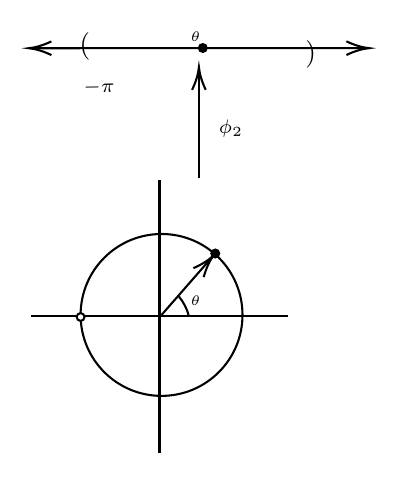
\begin{tikzpicture}[x=0.75pt,y=0.75pt,yscale=-1,xscale=1]
%uncomment if require: \path (0,300); %set diagram left start at 0, and has height of 300

\draw   (258,177.73) -- (382,177.73)(320,112) -- (320,243.47) ;
%Straight Lines [id:da1268514518445265] 
\draw    (259,48.5) -- (419,48.47) ;
\draw [shift={(421,48.47)}, rotate = 179.99] [color={rgb, 255:red, 0; green, 0; blue, 0 }  ][line width=0.75]    (10.93,-3.29) .. controls (6.95,-1.4) and (3.31,-0.3) .. (0,0) .. controls (3.31,0.3) and (6.95,1.4) .. (10.93,3.29)   ;
\draw [shift={(257,48.5)}, rotate = 359.99] [color={rgb, 255:red, 0; green, 0; blue, 0 }  ][line width=0.75]    (10.93,-3.29) .. controls (6.95,-1.4) and (3.31,-0.3) .. (0,0) .. controls (3.31,0.3) and (6.95,1.4) .. (10.93,3.29)   ;
%Shape: Circle [id:dp7024113415149893] 
\draw   (282,177) .. controls (282,155.46) and (299.46,138) .. (321,138) .. controls (342.54,138) and (360,155.46) .. (360,177) .. controls (360,198.54) and (342.54,216) .. (321,216) .. controls (299.46,216) and (282,198.54) .. (282,177) -- cycle ;
%Shape: Circle [id:dp9335574434248441] 
\draw  [fill={rgb, 255:red, 255; green, 255; blue, 255 }  ,fill opacity=1 ] (280.12,178) .. controls (280.12,176.96) and (280.96,176.12) .. (282,176.12) .. controls (283.04,176.12) and (283.88,176.96) .. (283.88,178) .. controls (283.88,179.04) and (283.04,179.88) .. (282,179.88) .. controls (280.96,179.88) and (280.12,179.04) .. (280.12,178) -- cycle ;
%Straight Lines [id:da8252578804556748] 
\draw    (321,177) -- (344.68,149.91) ;
\draw [shift={(346,148.4)}, rotate = 131.16] [color={rgb, 255:red, 0; green, 0; blue, 0 }  ][line width=0.75]    (10.93,-3.29) .. controls (6.95,-1.4) and (3.31,-0.3) .. (0,0) .. controls (3.31,0.3) and (6.95,1.4) .. (10.93,3.29)   ;
%Shape: Arc [id:dp3291144774774024] 
\draw  [draw opacity=0] (329.32,168.07) .. controls (331.56,170.78) and (333.24,173.99) .. (334.17,177.52) -- (311.15,183.94) -- cycle ; \draw   (329.32,168.07) .. controls (331.56,170.78) and (333.24,173.99) .. (334.17,177.52) ;  
%Straight Lines [id:da3615704984807794] 
\draw    (339,110.87) -- (339,59.62) ;
\draw [shift={(339,57.62)}, rotate = 90] [color={rgb, 255:red, 0; green, 0; blue, 0 }  ][line width=0.75]    (10.93,-3.29) .. controls (6.95,-1.4) and (3.31,-0.3) .. (0,0) .. controls (3.31,0.3) and (6.95,1.4) .. (10.93,3.29)   ;
%Shape: Circle [id:dp19768643904648886] 
\draw  [fill={rgb, 255:red, 0; green, 0; blue, 0 }  ,fill opacity=1 ] (345,147.4) .. controls (345,146.36) and (345.84,145.52) .. (346.88,145.52) .. controls (347.92,145.52) and (348.77,146.36) .. (348.77,147.4) .. controls (348.77,148.44) and (347.92,149.28) .. (346.88,149.28) .. controls (345.84,149.28) and (345,148.44) .. (345,147.4) -- cycle ;
%Shape: Circle [id:dp2589693685269747] 
\draw  [fill={rgb, 255:red, 0; green, 0; blue, 0 }  ,fill opacity=1 ] (339,48.4) .. controls (339,47.36) and (339.84,46.52) .. (340.88,46.52) .. controls (341.92,46.52) and (342.77,47.36) .. (342.77,48.4) .. controls (342.77,49.44) and (341.92,50.28) .. (340.88,50.28) .. controls (339.84,50.28) and (339,49.44) .. (339,48.4) -- cycle ;

% Text Node
\draw (333.5,166.1) node [anchor=north west][inner sep=0.75pt]  [font=\tiny]  {$\theta $};
% Text Node

% Text Node
\draw (279.88,39.5) node [anchor=north west][inner sep=0.75pt]  [rotate=-359.08]  {$($};
% Text Node
\draw (396.98,59.62) node [anchor=north west][inner sep=0.75pt]  [rotate=-180.17]  {$($};
% Text Node
\draw (281.88,62.5) node [anchor=north west][inner sep=0.75pt]  [font=\scriptsize,rotate=-359.08]  {$-\pi $};
% Text Node
\draw (387.88,61.5) node [anchor=north west][inner sep=0.75pt]  [font=\scriptsize,rotate=-359.08]  {$\uppi $};
% Text Node
\draw (333.5,39.1) node [anchor=north west][inner sep=0.75pt]  [font=\tiny]  {$\theta $};
% Text Node
\draw (347.05,81.61) node [anchor=north west][inner sep=0.75pt]  [font=\scriptsize,rotate=-359.08]  {$\phi _{2}$};


\end{tikzpicture}

    \caption{Here the point $(-1,0)$ is removed and $\phi_2$ maps the rest of the circle to the interval $(-\pi,\pi)$.}
    \label{fig:circchart2}
  \end{subfigure}
  \caption{$\phi_1$ and $\phi_2$ are invertiable and continuous (easily seen).  The two charts intersect in the upper and lower semicircles (as the antipodal points are removed). The transition function is given by:
  \(\phi_1 \circ \phi_2^{-1}(\theta) = \begin{cases}   \theta  & \text{if } \theta\in (0, \pi) \\  \theta+2\pi & \text{if } \theta \in (-\pi, 0) \end{cases}\)which is \textit{smooth} on each of the semicircles as required. Thus this is a valid chart for the circle.}  
  
\end{figure}
\noindent
The same circle can be described by another chart using the stereographic projection, resulting in the \textbf{Mercator Atlas}. For this let us consider $U_1 = \mathbb{S}\backslash(0,1)$ and $U_2 = \mathbb{S}\backslash(0,-1)$. Then what we do is, we define maps $\phi_1: U_1 \rightarrow \mathbb{R}$ ($\phi_2:U_2 \rightarrow \mathbb{R}$) which maps a point $p\in U_1(U_2)$ to some point on the x-axis. This is called a stereographic projection.  Let us find explicit forms for these maps:
\begin{figure}[H]
  \centering
  

\tikzset{every picture/.style={line width=0.75pt}} %set default line width to 0.75pt        

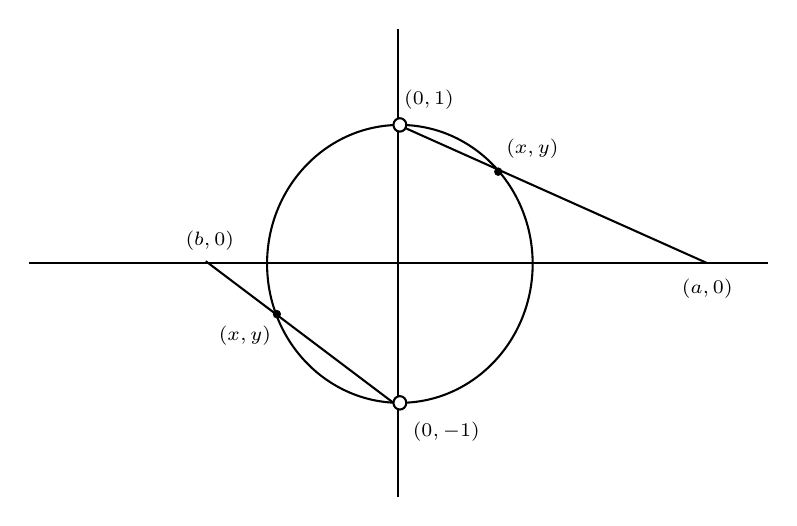
\begin{tikzpicture}[x=0.75pt,y=0.75pt,yscale=-1,xscale=1]
%uncomment if require: \path (0,300); %set diagram left start at 0, and has height of 300

%Straight Lines [id:da38416839783490875] 
\draw    (334.91,86.07) -- (479.47,150.76) ;
\draw   (153,150.84) -- (509,150.84)(331,38) -- (331,263.68) ;
%Shape: Ellipse [id:dp5420230958012913] 
\draw   (267.84,151.3) .. controls (267.84,114.32) and (296.48,84.35) .. (331.82,84.35) .. controls (367.16,84.35) and (395.8,114.32) .. (395.8,151.3) .. controls (395.8,188.27) and (367.16,218.25) .. (331.82,218.25) .. controls (296.48,218.25) and (267.84,188.27) .. (267.84,151.3) -- cycle ;
%Shape: Ellipse [id:dp36221512805207556] 
\draw  [fill={rgb, 255:red, 255; green, 255; blue, 255 }  ,fill opacity=1 ] (328.73,84.35) .. controls (328.73,82.56) and (330.11,81.12) .. (331.82,81.12) .. controls (333.53,81.12) and (334.91,82.56) .. (334.91,84.35) .. controls (334.91,86.14) and (333.53,87.58) .. (331.82,87.58) .. controls (330.11,87.58) and (328.73,86.14) .. (328.73,84.35) -- cycle ;
%Shape: Ellipse [id:dp009187332823011762] 
\draw  [fill={rgb, 255:red, 0; green, 0; blue, 0 }  ,fill opacity=1 ] (377.76,106.87) .. controls (377.76,106.03) and (378.4,105.35) .. (379.2,105.35) .. controls (380.01,105.35) and (380.65,106.03) .. (380.65,106.87) .. controls (380.65,107.7) and (380.01,108.38) .. (379.2,108.38) .. controls (378.4,108.38) and (377.76,107.7) .. (377.76,106.87) -- cycle ;
%Shape: Ellipse [id:dp6306749406268602] 
\draw  [fill={rgb, 255:red, 255; green, 255; blue, 255 }  ,fill opacity=1 ] (328.73,218.25) .. controls (328.73,216.46) and (330.11,215.02) .. (331.82,215.02) .. controls (333.53,215.02) and (334.91,216.46) .. (334.91,218.25) .. controls (334.91,220.03) and (333.53,221.48) .. (331.82,221.48) .. controls (330.11,221.48) and (328.73,220.03) .. (328.73,218.25) -- cycle ;
%Straight Lines [id:da9139964805053054] 
\draw    (328.73,218.25) -- (238.31,150.01) ;
%Shape: Ellipse [id:dp5109010146737958] 
\draw  [fill={rgb, 255:red, 0; green, 0; blue, 0 }  ,fill opacity=1 ] (271.12,175.53) .. controls (271.12,174.7) and (271.77,174.02) .. (272.57,174.02) .. controls (273.37,174.02) and (274.02,174.7) .. (274.02,175.53) .. controls (274.02,176.37) and (273.37,177.05) .. (272.57,177.05) .. controls (271.77,177.05) and (271.12,176.37) .. (271.12,175.53) -- cycle ;

% Text Node
\draw (381.6,89.84) node [anchor=north west][inner sep=0.75pt]  [font=\scriptsize]  {$( x,y)$};
% Text Node
\draw (243.09,179.57) node [anchor=north west][inner sep=0.75pt]  [font=\scriptsize]  {$( x,y)$};
% Text Node
\draw (332.38,65.98) node [anchor=north west][inner sep=0.75pt]  [font=\scriptsize]  {$( 0,1)$};
% Text Node
\draw (336.57,225.97) node [anchor=north west][inner sep=0.75pt]  [font=\scriptsize]  {$( 0,-1)$};
% Text Node
\draw (466.24,156.85) node [anchor=north west][inner sep=0.75pt]  [font=\scriptsize]  {$( a,0)$};
% Text Node
\draw (227.07,134.13) node [anchor=north west][inner sep=0.75pt]  [font=\scriptsize]  {$( b,0)$};


\end{tikzpicture}

  \caption{Stereographic projection of the circle} 
\end{figure}
\noindent
In the above picture, the equation of the straight line for $\phi_1$ is given by:
$$\frac{y-1}{x-0} = \frac{0-y}{a-x}$$ from where we obtain $a=\frac{x}{1-y}$. Similarly, we obtain $b = \frac{x}{1+y}$. Then what we have is $(x,y) \mapsto \frac{x}{1-y}$ (we take only the x-component since y-component is always 0 and thus the codomain is a real number) for $\phi_1$ and $(x,y) \mapsto \frac{x}{1+y}$ for $\phi_2$.  Suppose we are given a point \( (t, 0) \in \mathbb{R} \times \{0\} \), and we want to compute the inverse image under the stereographic projection \( \varphi_1^{-1} \).\\[0.2cm]
We are given that \( \varphi_1(x, y) = \dfrac{x}{1 - y} = t \). Solving for \( x \), we get:
\[
x = t(1 - y)
\]
Substitute this into the unit circle equation \( x^2 + y^2 = 1 \):
\begin{align*}
x^2 + y^2 &= 1 \\
\implies \ t^2(1 - y)^2 + y^2 &= 1 \\
\implies \ t^2(1 - 2y + y^2) + y^2 &= 1 \\
\implies \ t^2 - 2t^2 y + t^2 y^2 + y^2 &= 1 \\
\implies \ (1 + t^2)y^2 - 2t^2 y + (t^2 - 1) &= 0
\end{align*}
This is a quadratic in \( y \). Solving it gives:
\[
y = \frac{2t^2 \pm \sqrt{4}}{2(1 + t^2)} = \frac{t^2 \pm 1}{t^2 + 1}
\]
So the two roots are:
\[
y = 1, \quad y = \frac{t^2 - 1}{t^2 + 1}
\]
Since \( y = 1 \) corresponds to the north pole (which is excluded from the domain of \( \varphi_1 \)), we discard it. Thus, we have:
\[
y = \frac{t^2 - 1}{t^2 + 1}
\]
Now substitute back to find \( x \):
\begin{align*}
x &= t(1 - y) = t \left(1 - \frac{t^2 - 1}{t^2 + 1} \right)
= t \left( \frac{(t^2 + 1) - (t^2 - 1)}{t^2 + 1} \right)
= t \left( \frac{2}{t^2 + 1} \right)
= \frac{2t}{t^2 + 1}
\end{align*}
Hence, the inverse map \( \varphi_1^{-1}: \mathbb{R} \to S^1 \setminus \{(0,1)\} \) is given by:
\[
\boxed{
\varphi_1^{-1}(t) = \left( \frac{2t}{1 + t^2}, \frac{t^2 - 1}{1 + t^2} \right)
}
\]
Note that this map is continuous and hence this is a homeomorphism. Similarly, we can prove it for $\phi_2$ also. Now, if we take a point from the intersection, $U_1\bigcap U_2$ (that is, the circle without the poles), then we can never obtain the point $(0,0)$ since both maps give $(0,0)$ only when one of the input is along the y-xis. Thus, $\phi_1(U_1\bigcap U_2) = \mathbb{R}\backslash 0, \phi_2(U_1\bigcap U_2) = \mathbb{R}\backslash 0$. Now let's see the transition map: 
$$\phi_2 \circ \phi_1^{-1} = \phi_2 \brac{\frac{2t}{1+t^2}, \frac{t^2-1}{t^2+1}} = \frac{\frac{2t}{t^2+1}}{\frac{t^2-1}{t^2+1}-1} = \frac{2t}{2t^2} = \frac{1}{t}$$ which is smooth on $\mathbb{R}\backslash 0 $. Similarly for the other case also, we can show. Thus $\{(U_1, \varphi_1), (U_2, \varphi_2)\}$ for an atlas for the circle and is called the Mercator Atlas. 
Similarly we can prove that the $n$-dimensional sphere is a manifold. \\[0.3cm]
\textbf{Product Manifold:}\\[0.2cm]
Let $\mathcal{M}$ be an $m$-dimensional manifold with atlas $\{U_i,\varphi_i\}$ and $\mathcal{N}$ be an $n$-dimensional manifold with atlas $\{V_i,\psi_i\}$, then we define the product manifold as an $(m+n)-$ dimensional manifold with atlas $\{U_i\times V_j, (\phi_i , \psi_j)\}$. So basically we took the Cartesian product of the two coordinate neighbourhoods to define the new neighbourhood and then used the ordered pair of the two homeomorphisms to define the new coordinate function. \\[0.3cm]
\textit{Example.} The torus is a product manifold of two circles, that is, $T^2 = \mathbb{S}^1\times \mathbb{S}^1$. Note that by our definition, it is a two $(1+1)$ dimensional manifold. We can generalise the notion of torus by taking multiple product of circles: $$T^n = \underbrace{\mathbb{S}^1\times \mathbb{S}^1\times \cdots \times \mathbb{S}^1}_n$$ 
\subsubsection{Differentiable Maps}
\begin{definition}[Differentiable Map]
  A map $f: \mathcal{M}_m \to \mathcal{N}_n$ between two manifolds is \textit{differentiable} at $p$ if for any charts $(U,\phi)$ on $\mathcal{M}$ and $(V,\psi)$ on $\mathcal{N}$ (where $p\in U$ and $f(p)\in V$), the map $$\psi \circ f \circ \phi^{-1}: \mathbb{R}^m \rightarrow \mathbb{R}^n$$
  is a smooth map, that is, the map belongs to $C^\infty$, that is, infinitely continuously differentiable. 
\end{definition}
WTH...\emoji{worried-face} what is this weird map that we want to be smooth? Let us see in more details. So, what does $f$ do? It is a map from manifold $\mathcal{M}$ to manifold $\mathcal{N}$ and it maps $p \mapsto f(p)$. So far good...Now, we know that we can obtain coordinate representations using the homeomorphisms. Let them be:
$$\phi(p) \equiv \{x^\mu\}\quad\quad\quad \psi(f(p)) \equiv \{y^\alpha\}$$
So what $\psi \circ f \circ \phi^{-1}$ does is, it takes a vector from $\mathbb{R}^m$, sends it back to the manifold $\mathcal{M}$, applies $f$ to it to send it to manifold $\mathcal{N}$ and then sends it to $\mathbb{R}^n$, so finally we obtain a $n$ element output from $m$ element input, using $f$. So this is just the usual map like what we write $\veb{y} = f(\veb{x})$. Lol, this is nothing but the differentiability of a function, albeit in a more stylish (and appropriate) way.
\begin{figure}[H]
  \centering 
  

\tikzset{every picture/.style={line width=0.75pt}} %set default line width to 0.75pt        

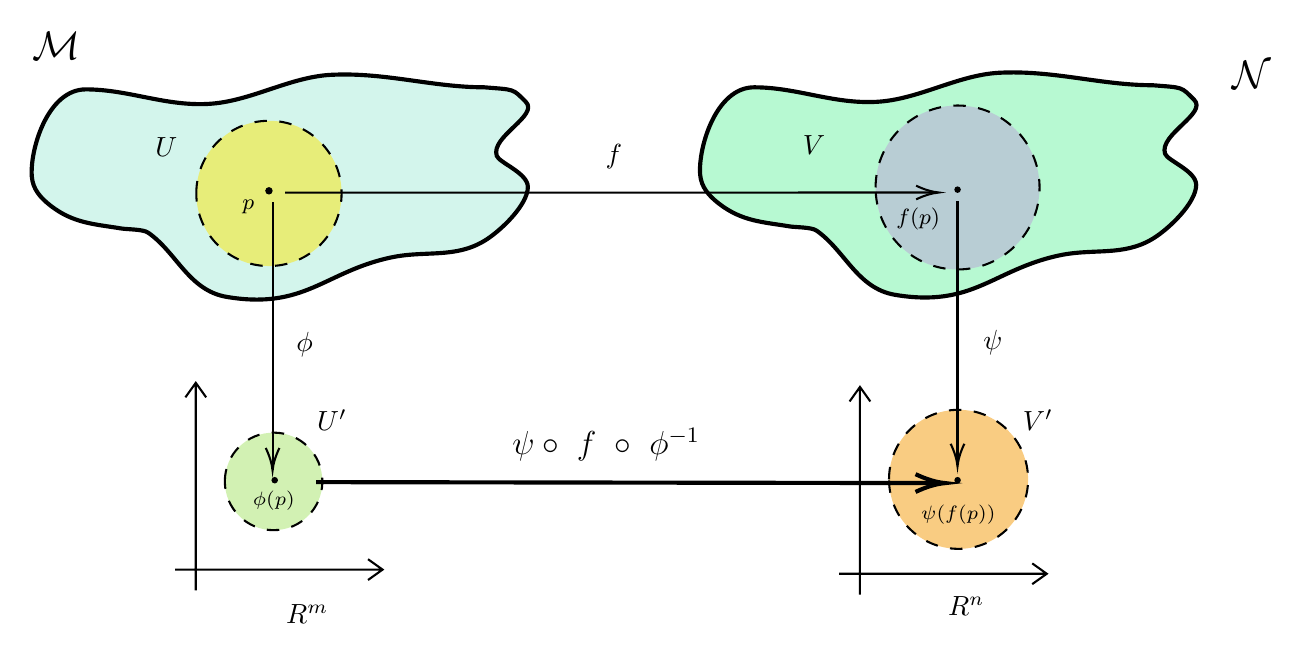
\begin{tikzpicture}[x=0.75pt,y=0.75pt,yscale=-1,xscale=1]
%uncomment if require: \path (0,351); %set diagram left start at 0, and has height of 351

%Shape: Circle [id:dp4604718091966047] 
\draw  [fill={rgb, 255:red, 184; green, 233; blue, 134 }  ,fill opacity=0.63 ][dash pattern={on 4.5pt off 4.5pt}] (119,224.5) .. controls (119,211.52) and (129.52,201) .. (142.5,201) .. controls (155.48,201) and (166,211.52) .. (166,224.5) .. controls (166,237.48) and (155.48,248) .. (142.5,248) .. controls (129.52,248) and (119,237.48) .. (119,224.5) -- cycle ;
%Shape: Circle [id:dp3442356821329243] 
\draw  [fill={rgb, 255:red, 245; green, 166; blue, 35 }  ,fill opacity=0.57 ][dash pattern={on 4.5pt off 4.5pt}] (439,223.5) .. controls (439,205) and (454,190) .. (472.5,190) .. controls (491,190) and (506,205) .. (506,223.5) .. controls (506,242) and (491,257) .. (472.5,257) .. controls (454,257) and (439,242) .. (439,223.5) -- cycle ;
%Curve Lines [id:da8514602322717827] 
\draw [fill={rgb, 255:red, 8; green, 233; blue, 99 }  ,fill opacity=0.29 ][line width=1.5] [line join = round][line cap = round]   (566,33.63) .. controls (541.07,33.63) and (518.02,26.24) .. (492,27.63) .. controls (471.94,28.71) and (453.25,40.57) .. (433,41.63) .. controls (411.98,42.74) and (394.57,34.63) .. (374,34.63) .. controls (355.59,34.63) and (347.01,63.73) .. (348,76.63) .. controls (348.47,82.7) and (352.18,86.88) .. (357,90.63) .. controls (368.08,99.25) and (378.24,99.51) .. (391,101.63) .. controls (393.95,102.13) and (401.58,101.96) .. (404,103.63) .. controls (417.88,113.24) and (423.56,131.56) .. (442,134.63) .. controls (479.55,140.89) and (489.14,122.46) .. (521,115.63) .. controls (537.52,112.09) and (551.69,116.22) .. (566,107.63) .. controls (573.71,103.01) and (587,90.32) .. (587,81.63) .. controls (587,74.9) and (573.1,69.94) .. (572,66.63) .. controls (568.91,57.36) and (592.59,47.22) .. (586,40.63) .. controls (579.54,34.17) and (581,34.85) .. (566,33.63) -- cycle ;
%Curve Lines [id:da2024130737434997] 
\draw [fill={rgb, 255:red, 211; green, 245; blue, 236 }  ,fill opacity=1 ][line width=1.5] [line join = round][line cap = round]   (244,34.63) .. controls (219.07,34.63) and (196.02,27.24) .. (170,28.63) .. controls (149.94,29.71) and (131.25,41.57) .. (111,42.63) .. controls (89.98,43.74) and (72.57,35.63) .. (52,35.63) .. controls (33.59,35.63) and (25.01,64.73) .. (26,77.63) .. controls (26.47,83.7) and (30.18,87.88) .. (35,91.63) .. controls (46.08,100.25) and (56.24,100.51) .. (69,102.63) .. controls (71.95,103.13) and (79.58,102.96) .. (82,104.63) .. controls (95.88,114.24) and (101.56,132.56) .. (120,135.63) .. controls (157.55,141.89) and (167.14,123.46) .. (199,116.63) .. controls (215.52,113.09) and (229.69,117.22) .. (244,108.63) .. controls (251.71,104.01) and (265,91.32) .. (265,82.63) .. controls (265,75.9) and (251.1,70.94) .. (250,67.63) .. controls (246.91,58.36) and (270.59,48.22) .. (264,41.63) .. controls (257.54,35.17) and (259,35.85) .. (244,34.63) -- cycle ;
%Shape: Circle [id:dp06624735745121968] 
\draw  [fill={rgb, 255:red, 248; green, 231; blue, 28 }  ,fill opacity=0.55 ][dash pattern={on 4.5pt off 4.5pt}] (105.25,85.75) .. controls (105.25,66.42) and (120.92,50.75) .. (140.25,50.75) .. controls (159.58,50.75) and (175.25,66.42) .. (175.25,85.75) .. controls (175.25,105.08) and (159.58,120.75) .. (140.25,120.75) .. controls (120.92,120.75) and (105.25,105.08) .. (105.25,85.75) -- cycle ;
%Shape: Circle [id:dp05380630291243382] 
\draw  [fill={rgb, 255:red, 189; green, 16; blue, 224 }  ,fill opacity=0.19 ][dash pattern={on 4.5pt off 4.5pt}] (432.53,82.9) .. controls (432.53,61.08) and (450.22,43.4) .. (472.03,43.4) .. controls (493.85,43.4) and (511.53,61.08) .. (511.53,82.9) .. controls (511.53,104.72) and (493.85,122.4) .. (472.03,122.4) .. controls (450.22,122.4) and (432.53,104.72) .. (432.53,82.9) -- cycle ;
%Straight Lines [id:da795651220900737] 
\draw    (142,90.08) -- (142,217.32) ;
\draw [shift={(142,219.32)}, rotate = 270] [color={rgb, 255:red, 0; green, 0; blue, 0 }  ][line width=0.75]    (10.93,-3.29) .. controls (6.95,-1.4) and (3.31,-0.3) .. (0,0) .. controls (3.31,0.3) and (6.95,1.4) .. (10.93,3.29)   ;
%Straight Lines [id:da47228720125648727] 
\draw    (472,89.32) -- (472,215.32) ;
\draw [shift={(472,217.32)}, rotate = 270] [color={rgb, 255:red, 0; green, 0; blue, 0 }  ][line width=0.75]    (10.93,-3.29) .. controls (6.95,-1.4) and (3.31,-0.3) .. (0,0) .. controls (3.31,0.3) and (6.95,1.4) .. (10.93,3.29)   ;
%Shape: Axis 2D [id:dp4084611261773249] 
\draw  (95,267) -- (195,267)(105,177) -- (105,277) (188,262) -- (195,267) -- (188,272) (100,184) -- (105,177) -- (110,184)  ;
%Shape: Axis 2D [id:dp12556457670089383] 
\draw  (415,269) -- (515,269)(425,179) -- (425,279) (508,264) -- (515,269) -- (508,274) (420,186) -- (425,179) -- (430,186)  ;
%Straight Lines [id:da43480740287261954] 
\draw [line width=1.5]    (463,225.31) -- (163,224.85) ;
\draw [shift={(466,225.32)}, rotate = 180.09] [color={rgb, 255:red, 0; green, 0; blue, 0 }  ][line width=1.5]    (14.21,-4.28) .. controls (9.04,-1.82) and (4.3,-0.39) .. (0,0) .. controls (4.3,0.39) and (9.04,1.82) .. (14.21,4.28)   ;
%Shape: Circle [id:dp17641131819546774] 
\draw  [fill={rgb, 255:red, 0; green, 0; blue, 0 }  ,fill opacity=1 ] (139,84.5) .. controls (139,83.81) and (139.56,83.25) .. (140.25,83.25) .. controls (140.94,83.25) and (141.5,83.81) .. (141.5,84.5) .. controls (141.5,85.19) and (140.94,85.75) .. (140.25,85.75) .. controls (139.56,85.75) and (139,85.19) .. (139,84.5) -- cycle ;
%Shape: Circle [id:dp9098380916442051] 
\draw  [fill={rgb, 255:red, 0; green, 0; blue, 0 }  ,fill opacity=1 ] (142,223.93) .. controls (142,224.5) and (142.46,224.97) .. (143.03,224.97) .. controls (143.6,224.97) and (144.07,224.5) .. (144.07,223.93) .. controls (144.07,223.36) and (143.6,222.9) .. (143.03,222.9) .. controls (142.46,222.9) and (142,223.36) .. (142,223.93) -- cycle ;
%Straight Lines [id:da12001174564982175] 
\draw    (148,85.37) -- (461,85.32) ;
\draw [shift={(463,85.32)}, rotate = 179.99] [color={rgb, 255:red, 0; green, 0; blue, 0 }  ][line width=0.75]    (10.93,-3.29) .. controls (6.95,-1.4) and (3.31,-0.3) .. (0,0) .. controls (3.31,0.3) and (6.95,1.4) .. (10.93,3.29)   ;
%Shape: Circle [id:dp6218977499267407] 
\draw  [fill={rgb, 255:red, 0; green, 0; blue, 0 }  ,fill opacity=1 ] (471,83.93) .. controls (471,84.5) and (471.46,84.97) .. (472.03,84.97) .. controls (472.6,84.97) and (473.07,84.5) .. (473.07,83.93) .. controls (473.07,83.36) and (472.6,82.9) .. (472.03,82.9) .. controls (471.46,82.9) and (471,83.36) .. (471,83.93) -- cycle ;
%Shape: Circle [id:dp25390351977169645] 
\draw  [fill={rgb, 255:red, 0; green, 0; blue, 0 }  ,fill opacity=1 ] (471,223.93) .. controls (471,224.5) and (471.46,224.97) .. (472.03,224.97) .. controls (472.6,224.97) and (473.07,224.5) .. (473.07,223.93) .. controls (473.07,223.36) and (472.6,222.9) .. (472.03,222.9) .. controls (471.46,222.9) and (471,223.36) .. (471,223.93) -- cycle ;

% Text Node
\draw (84,57.4) node [anchor=north west][inner sep=0.75pt]    {$U$};
% Text Node
\draw (147,282.4) node [anchor=north west][inner sep=0.75pt]    {$\mathbb{R}^{m}$};
% Text Node
\draw (466,278.4) node [anchor=north west][inner sep=0.75pt]    {$\mathbb{R}^{n}$};
% Text Node
\draw (162,188.4) node [anchor=north west][inner sep=0.75pt]    {$U '$};
% Text Node
\draw (502,188.4) node [anchor=north west][inner sep=0.75pt]    {$V'$};
% Text Node
\draw (152,151.4) node [anchor=north west][inner sep=0.75pt]    {$\phi $};
% Text Node
\draw (453,234.4) node [anchor=north west][inner sep=0.75pt]  [font=\scriptsize]  {$\psi ( f( p))$};
% Text Node
\draw (256,197.4) node [anchor=north west][inner sep=0.75pt]  [font=\large]  {$\psi \circ \ f\ \circ \ \phi ^{-1}$};
% Text Node
\draw (25,6.4) node [anchor=north west][inner sep=0.75pt]  [font=\Large]  {$\mathcal{M}$};
% Text Node
\draw (396,56.4) node [anchor=north west][inner sep=0.75pt]    {$V$};
% Text Node
\draw (126,87.4) node [anchor=north west][inner sep=0.75pt]  [font=\footnotesize]  {$p$};
% Text Node
\draw (131,227.4) node [anchor=north west][inner sep=0.75pt]  [font=\scriptsize]  {$\phi ( p)$};
% Text Node
\draw (441,91.4) node [anchor=north west][inner sep=0.75pt]  [font=\footnotesize]  {$f( p)$};
% Text Node
\draw (603,20.4) node [anchor=north west][inner sep=0.75pt]  [font=\Large]  {$\mathcal{N}$};
% Text Node
\draw (483,150.4) node [anchor=north west][inner sep=0.75pt]    {$\psi $};
% Text Node
\draw (301,60.4) node [anchor=north west][inner sep=0.75pt]    {$f$};


\end{tikzpicture}

  \caption{Representation of a differentiable map}
\end{figure}
\noindent
Next to come to another \textit{-morphism} related to the differentiable manifolds. 
\begin{definition}[Diffeomorphism]
  Let $f: \mathcal{M}_m \rightarrow \mathcal{N}_n$ be a homeomorphism and $\psi$ and $\phi$ be the coordinate functions as defined before. If $\psi\circ f\circ\phi^{-1}$ is invertible and both $\psi\circ f\circ\phi^{-1}$ and its inverse $\phi\circ f^{-1}\circ\psi^{-1}$ are smooth maps, then $f$ is called a \textit{diffeomorphism}. The manifolds are then said to be diffeomorphic to each other.
\end{definition}
Well, we had earlier seen that homeomorphisms characterise spaces which can be `continuously' deformed into each other. Diffeomorphism does one thing extra, it characterises spaces which are transformed `smoothly' into each other. Evidently, a diffeomorphism is also a homeomorphism. If two spaces a diffeomorphic, then their dimensions are same, that is $\dim \mathcal{M} = \dim \mathcal{N}$\\[0.3cm]
The set of diffeomorphisms $f:\mathcal{M}\rightarrow\mathcal{M}$ is a group and is denoted by $\mathrm{Diff}(\mathcal{M})$. 
\subsubsection{Pullback of a function}
\begin{figure}[H]
  \centering
  

\tikzset{every picture/.style={line width=0.75pt}} %set default line width to 0.75pt        

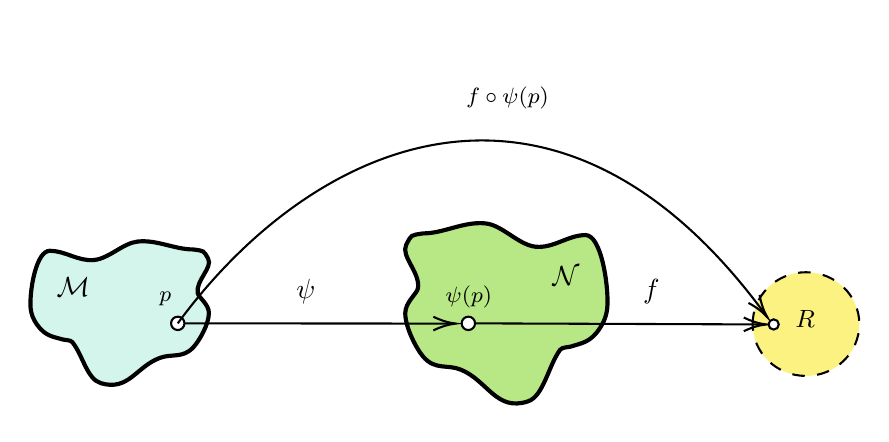
\begin{tikzpicture}[x=0.75pt,y=0.75pt,yscale=-1,xscale=1]
%uncomment if require: \path (0,230); %set diagram left start at 0, and has height of 230

%Shape: Boxed Bezier Curve [id:dp548963754265211] 
\draw [fill={rgb, 255:red, 211; green, 245; blue, 236 }  ,fill opacity=1 ][line width=1.5]    (171.39,104.78) .. controls (162.43,104.78) and (154.14,100.07) .. (144.78,100.95) .. controls (137.56,101.64) and (130.84,109.2) .. (123.56,109.88) .. controls (116,110.59) and (109.74,105.42) .. (102.34,105.42) .. controls (95.72,105.42) and (92.63,123.97) .. (92.99,132.2) .. controls (93.16,136.07) and (94.49,138.74) .. (96.23,141.13) .. controls (100.21,146.62) and (103.87,146.79) .. (108.45,148.14) .. controls (109.52,148.46) and (112.26,148.35) .. (113.13,149.42) .. controls (118.12,155.54) and (120.17,167.23) .. (126.8,169.19) .. controls (140.3,173.18) and (143.75,161.42) .. (155.21,157.07) .. controls (161.15,154.81) and (166.24,157.45) .. (171.39,151.97) .. controls (174.16,149.02) and (178.94,140.93) .. (178.94,135.39) .. controls (178.94,131.1) and (173.94,127.93) .. (173.55,125.82) .. controls (172.44,119.91) and (180.95,113.45) .. (178.58,109.24) .. controls (176.26,105.12) and (176.78,105.56) .. (171.39,104.78) -- cycle ;
%Shape: Ellipse [id:dp29255012486968357] 
\draw  [fill={rgb, 255:red, 248; green, 231; blue, 28 }  ,fill opacity=0.55 ][dash pattern={on 4.5pt off 4.5pt}] (440.91,140.74) .. controls (440.91,126.94) and (452.42,115.76) .. (466.62,115.76) .. controls (480.81,115.76) and (492.32,126.94) .. (492.32,140.74) .. controls (492.32,154.54) and (480.81,165.72) .. (466.62,165.72) .. controls (452.42,165.72) and (440.91,154.54) .. (440.91,140.74) -- cycle ;
%Shape: Boxed Bezier Curve [id:dp2261869946937909] 
\draw [fill={rgb, 255:red, 126; green, 211; blue, 33 }  ,fill opacity=0.55 ][line width=1.5]    (282.11,97.05) .. controls (292.27,97.05) and (301.66,91.12) .. (312.27,92.24) .. controls (320.45,93.1) and (328.07,102.61) .. (336.32,103.46) .. controls (344.89,104.35) and (351.99,97.85) .. (360.37,97.85) .. controls (367.88,97.85) and (371.37,121.16) .. (370.97,131.5) .. controls (370.78,136.36) and (369.27,139.71) .. (367.3,142.72) .. controls (362.78,149.63) and (358.64,149.83) .. (353.44,151.54) .. controls (352.24,151.93) and (349.13,151.8) .. (348.14,153.14) .. controls (342.49,160.84) and (340.17,175.52) .. (332.65,177.98) .. controls (317.35,182.99) and (313.44,168.22) .. (300.45,162.75) .. controls (293.72,159.92) and (287.94,163.23) .. (282.11,156.34) .. controls (278.97,152.64) and (273.55,142.47) .. (273.55,135.51) .. controls (273.55,130.12) and (279.21,126.14) .. (279.66,123.49) .. controls (280.92,116.06) and (271.27,107.94) .. (273.96,102.66) .. controls (276.59,97.48) and (275.99,98.02) .. (282.11,97.05) -- cycle ;
%Straight Lines [id:da573620974924035] 
\draw    (163.94,140.39) -- (296,140.5) ;
\draw [shift={(298,140.5)}, rotate = 180.05] [color={rgb, 255:red, 0; green, 0; blue, 0 }  ][line width=0.75]    (10.93,-3.29) .. controls (6.95,-1.4) and (3.31,-0.3) .. (0,0) .. controls (3.31,0.3) and (6.95,1.4) .. (10.93,3.29)   ;
%Straight Lines [id:da00667541340455724] 
\draw    (307.17,140.39) -- (445.58,140.91) ;
\draw [shift={(447.58,140.92)}, rotate = 180.22] [color={rgb, 255:red, 0; green, 0; blue, 0 }  ][line width=0.75]    (10.93,-3.29) .. controls (6.95,-1.4) and (3.31,-0.3) .. (0,0) .. controls (3.31,0.3) and (6.95,1.4) .. (10.93,3.29)   ;
%Shape: Circle [id:dp8370900540926526] 
\draw  [fill={rgb, 255:red, 255; green, 255; blue, 255 }  ,fill opacity=1 ] (160.72,140.39) .. controls (160.72,138.61) and (162.16,137.16) .. (163.94,137.16) .. controls (165.72,137.16) and (167.17,138.61) .. (167.17,140.39) .. controls (167.17,142.17) and (165.72,143.61) .. (163.94,143.61) .. controls (162.16,143.61) and (160.72,142.17) .. (160.72,140.39) -- cycle ;
%Shape: Circle [id:dp1381101300882457] 
\draw  [fill={rgb, 255:red, 255; green, 255; blue, 255 }  ,fill opacity=1 ] (300.72,140.39) .. controls (300.72,138.61) and (302.16,137.16) .. (303.94,137.16) .. controls (305.72,137.16) and (307.17,138.61) .. (307.17,140.39) .. controls (307.17,142.17) and (305.72,143.61) .. (303.94,143.61) .. controls (302.16,143.61) and (300.72,142.17) .. (300.72,140.39) -- cycle ;
%Curve Lines [id:da7070782507909167] 
\draw    (163.94,140.39) .. controls (229,51.7) and (347,-1.57) .. (448,137.45) ;
\draw [shift={(448,137.45)}, rotate = 234] [color={rgb, 255:red, 0; green, 0; blue, 0 }  ][line width=0.75]    (10.93,-3.29) .. controls (6.95,-1.4) and (3.31,-0.3) .. (0,0) .. controls (3.31,0.3) and (6.95,1.4) .. (10.93,3.29)   ;
%Shape: Circle [id:dp9897406803094917] 
\draw  [fill={rgb, 255:red, 255; green, 255; blue, 255 }  ,fill opacity=1 ] (453.52,140.92) .. controls (453.52,139.55) and (452.41,138.45) .. (451.05,138.45) .. controls (449.69,138.45) and (448.58,139.55) .. (448.58,140.92) .. controls (448.58,142.28) and (449.69,143.38) .. (451.05,143.38) .. controls (452.41,143.38) and (453.52,142.28) .. (453.52,140.92) -- cycle ;

% Text Node
\draw (104.02,116.65) node [anchor=north west][inner sep=0.75pt]  [font=\normalsize]  {$\mathcal{M}$};
% Text Node
\draw (219.61,117.78) node [anchor=north west][inner sep=0.75pt]    {$\psi $};
% Text Node
\draw (343.02,111.65) node [anchor=north west][inner sep=0.75pt]  [font=\normalsize]  {$\mathcal{N}$};
% Text Node
\draw (386.61,117.78) node [anchor=north west][inner sep=0.75pt]    {$f$};
% Text Node
\draw (460.02,132.65) node [anchor=north west][inner sep=0.75pt]  [font=\small]  {$\mathbb{R}$};
% Text Node
\draw (153.55,123.85) node [anchor=north west][inner sep=0.75pt]  [font=\footnotesize]  {$p$};
% Text Node
\draw (291.55,120.85) node [anchor=north west][inner sep=0.75pt]  [font=\footnotesize]  {$\psi ( p)$};
% Text Node
\draw (301.55,24.85) node [anchor=north west][inner sep=0.75pt]  [font=\footnotesize]  {$f\circ \psi ( p)$};


\end{tikzpicture}

\end{figure}
Given a smooth map $\psi:\SM \rightarrow \SN$ and $f\in C^\infty(\SN)$, the pullback of $f$ along $\psi$ is defined to be:
$$\psi^*f\equiv f\circ \psi : \SM\rightarrow \re$$
Since $f$ and $\psi$ both are smooth maps, their composition (which is a real-valued function) is too! Thus, $\psi^*$ can be thought of as a map from $C^\infty(\SN) \rightarrow C^\infty(\SM)$. Thus, it sort of `pulls back' to the original manifold from which $\psi$ was defined. \footnote{This has something to do dual space and one-forms also, apparently, which maybe seen later.} Also, note the following properties of the pullback for two functions $f,g \in C^\infty(\SN)$:
\begin{itemize}
  \item $\psi^*(f+g)(p) \equiv (f+g)\circ \psi(p) = f(\psi(p))+g(\psi(p)) = \psi^*f(p)+\psi^*g(p)$
  \item $\psi^*(fg)(p) = (fg)\circ \psi(p) = f(\psi(p))g(\psi(p)) = (\psi^*f(p))(\psi^*g(p))$
\end{itemize}
\subsubsection{Curves}
\begin{definition}[Curve]
  An open curve in an $m$-dimensional manifold $\mathcal{M}$ is a map $\sigma:(a,b)\rightarrow \mathcal{M}$ such that $a<0<b$ ($a$ and $b$ can be $\pm \infty$ also). A closed curve is a map $\sigma:\mathbb{S}^1\rightarrow \mathcal{M}$

\end{definition}
What this means is that suppose we take $t\in (a,b)$, then $\sigma(t)$ is a point on the manifold. As $t$ is varied in the interval, the points $\sigma(t)$ kinda resembles a trajectory (which we intuitively had called a `curve' so far). We had included zero in the interval for convenience. 
\subsubsection{Vectors}
In our usual sense, we imagine vectors as straight arrows drawn from the origin but in manifolds, which is `curved', firstly, straight arrows cannot be drawn in general and secondly, there is no origin from which the arrow can be drawn. If the arrow is `small' enough we can locally obtain something like a ``vector space''. Suppose the tail of the arrow is at a point $p\in \mathcal{M}$ and the tip is at a point $p'$ which is `close' to $p$, then the vector space can be approximated by the \textit{tangent space} at the point $p$. 
\subsection{Tangent Space}
Intuitively, if we use the word tangent space, we can think of some space which contains the tangent at a point of the manifold. Like in the following diagram: 
\begin{figure}[H]
  \centering 
  

\tikzset{every picture/.style={line width=0.75pt}} %set default line width to 0.75pt        

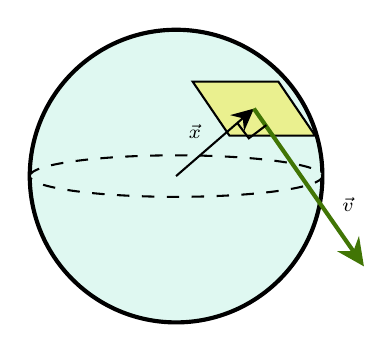
\begin{tikzpicture}[x=0.75pt,y=0.75pt,yscale=-1,xscale=1]
%uncomment if require: \path (0,300); %set diagram left start at 0, and has height of 300

%Shape: Circle [id:dp254606372765645] 
\draw  [fill={rgb, 255:red, 223; green, 248; blue, 241 }  ,fill opacity=1 ][line width=1.5]  (161,152.5) .. controls (161,113.56) and (192.56,82) .. (231.5,82) .. controls (270.44,82) and (302,113.56) .. (302,152.5) .. controls (302,191.44) and (270.44,223) .. (231.5,223) .. controls (192.56,223) and (161,191.44) .. (161,152.5) -- cycle ;
%Shape: Ellipse [id:dp7341918406156717] 
\draw  [fill={rgb, 255:red, 223; green, 248; blue, 241 }  ,fill opacity=1 ][dash pattern={on 4.5pt off 4.5pt}] (161,152.5) .. controls (161,146.98) and (192.56,142.5) .. (231.5,142.5) .. controls (270.44,142.5) and (302,146.98) .. (302,152.5) .. controls (302,158.02) and (270.44,162.5) .. (231.5,162.5) .. controls (192.56,162.5) and (161,158.02) .. (161,152.5) -- cycle ;
%Shape: Parallelogram [id:dp1888887727044548] 
\draw  [fill={rgb, 255:red, 248; green, 231; blue, 28 }  ,fill opacity=0.46 ] (280.8,107) -- (239.5,107) -- (257.2,133) -- (298.5,133) -- cycle ;
%Straight Lines [id:da5934768392694703] 
\draw    (231.5,152.5) -- (266.73,121.96) ;
\draw [shift={(269,120)}, rotate = 139.09] [fill={rgb, 255:red, 0; green, 0; blue, 0 }  ][line width=0.08]  [draw opacity=0] (10.72,-5.15) -- (0,0) -- (10.72,5.15) -- (7.12,0) -- cycle    ;
%Straight Lines [id:da12457450880261867] 
\draw [color={rgb, 255:red, 65; green, 117; blue, 5 }  ,draw opacity=1 ][line width=1.5]    (269,120) -- (319.71,192.72) ;
\draw [shift={(322,196)}, rotate = 235.11] [fill={rgb, 255:red, 65; green, 117; blue, 5 }  ,fill opacity=1 ][line width=0.08]  [draw opacity=0] (13.4,-6.43) -- (0,0) -- (13.4,6.44) -- (8.9,0) -- cycle    ;
%Shape: Right Angle [id:dp8028801232030925] 
\draw   (275,127.95) -- (266.56,134.3) -- (261.02,126.94) ;

% Text Node
\draw (236,126.4) node [anchor=north west][inner sep=0.75pt]  [font=\scriptsize]  {$\vec{x}$};
% Text Node
\draw (310,161.4) node [anchor=north west][inner sep=0.75pt]  [font=\scriptsize]  {$\vec{v}$};


\end{tikzpicture}

  \caption{A very badly made representation of a tangent space. Here a sphere is considered and from the centre of the sphere, a vector $\veb{x}$ is drawn and then, a plane is drawn which just touches the sphere at point $\veb{x}$. This constitutes the tangent plane. }
\end{figure}
\noindent
Note that since the tangent is always perpendicular to the vector $\veb{x}$, we can somewhat define the tangent space at the point $\veb{x}\in S^n \subset \mathbb{R}^{n+1}$ by: $$\mathrm{T}_{x}S^n = \{\veb{v}\in \mathbb{R}^{n+1}| \veb{x}\cdot \veb{v} = 0\}$$
See an apparent problem with this: This approach depends on the sphere being embedded in a higher dimension vector space and the tangent space being a specific linear subspace of this larger space. It would be better to find some `intrinsic' definition of tangent space which does not depend on this embedding of the manifold in a higher dimensional space.\\[0.3cm]
For this, we can think of the tangent vector as a tangent to a curve on the manifold. The vector is tangent to a curve on the manifold at point $\veb{x}$. Note that this curve lies on the manifold and hence the notion of a higher-dimensional embedding is done away with. 
\begin{figure}[H]
  \centering
  

\tikzset{every picture/.style={line width=0.75pt}} %set default line width to 0.75pt        

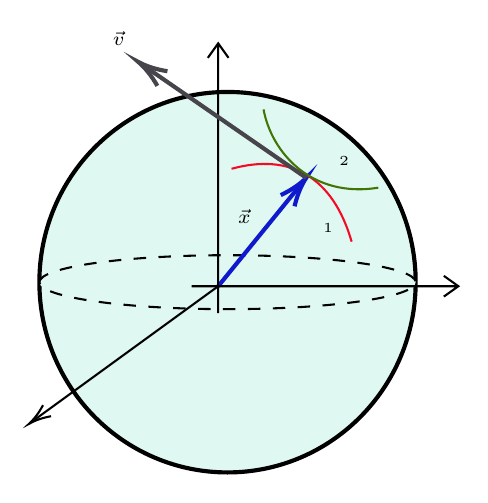
\begin{tikzpicture}[x=0.75pt,y=0.75pt,yscale=-1,xscale=1]
%uncomment if require: \path (0,300); %set diagram left start at 0, and has height of 300

%Shape: Ellipse [id:dp8621922183495604] 
\draw  [fill={rgb, 255:red, 223; green, 248; blue, 241 }  ,fill opacity=1 ][line width=1.5]  (171.14,159.71) .. controls (171.14,109.08) and (211.73,68.05) .. (261.79,68.05) .. controls (311.85,68.05) and (352.43,109.08) .. (352.43,159.71) .. controls (352.43,210.33) and (311.85,251.37) .. (261.79,251.37) .. controls (211.73,251.37) and (171.14,210.33) .. (171.14,159.71) -- cycle ;
%Shape: Ellipse [id:dp2859403935407516] 
\draw  [fill={rgb, 255:red, 223; green, 248; blue, 241 }  ,fill opacity=1 ][dash pattern={on 4.5pt off 4.5pt}] (171.14,159.71) .. controls (171.14,152.53) and (211.73,146.71) .. (261.79,146.71) .. controls (311.85,146.71) and (352.43,152.53) .. (352.43,159.71) .. controls (352.43,166.89) and (311.85,172.71) .. (261.79,172.71) .. controls (211.73,172.71) and (171.14,166.89) .. (171.14,159.71) -- cycle ;
%Straight Lines [id:da16269634334020433] 
\draw [color={rgb, 255:red, 15; green, 26; blue, 204 }  ,draw opacity=1 ][line width=1.5]    (257.29,161.66) -- (297.82,111.76) ;
\draw [shift={(299.71,109.43)}, rotate = 129.09] [color={rgb, 255:red, 15; green, 26; blue, 204 }  ,draw opacity=1 ][line width=1.5]    (14.21,-4.28) .. controls (9.04,-1.82) and (4.3,-0.39) .. (0,0) .. controls (4.3,0.39) and (9.04,1.82) .. (14.21,4.28)   ;
%Shape: Axis 2D [id:dp5781161322417953] 
\draw  (244.43,161.66) -- (373,161.66)(257.29,44.64) -- (257.29,174.66) (366,156.66) -- (373,161.66) -- (366,166.66) (252.29,51.64) -- (257.29,44.64) -- (262.29,51.64)  ;
%Straight Lines [id:da986530720222472] 
\draw    (257.29,161.66) -- (167.62,226.87) ;
\draw [shift={(166,228.05)}, rotate = 323.97] [color={rgb, 255:red, 0; green, 0; blue, 0 }  ][line width=0.75]    (10.93,-3.29) .. controls (6.95,-1.4) and (3.31,-0.3) .. (0,0) .. controls (3.31,0.3) and (6.95,1.4) .. (10.93,3.29)   ;
%Curve Lines [id:da2567673398245671] 
\draw [color={rgb, 255:red, 245; green, 10; blue, 38 }  ,draw opacity=1 ]   (263.71,105.08) .. controls (292,97.28) and (312.57,108.98) .. (321.57,140.18) ;
%Curve Lines [id:da2661789837245453] 
\draw [color={rgb, 255:red, 65; green, 117; blue, 5 }  ,draw opacity=1 ]   (279.14,76.48) .. controls (283,97.28) and (302.29,119.38) .. (334.43,114.18) ;
%Straight Lines [id:da53165768173298] 
\draw [color={rgb, 255:red, 71; green, 68; blue, 75 }  ,draw opacity=1 ][fill={rgb, 255:red, 61; green, 57; blue, 57 }  ,fill opacity=1 ][line width=1.5]    (299.71,109.43) -- (221.18,55.23) ;
\draw [shift={(218.71,53.53)}, rotate = 34.61] [color={rgb, 255:red, 71; green, 68; blue, 75 }  ,draw opacity=1 ][line width=1.5]    (14.21,-4.28) .. controls (9.04,-1.82) and (4.3,-0.39) .. (0,0) .. controls (4.3,0.39) and (9.04,1.82) .. (14.21,4.28)   ;

% Text Node
\draw (265.43,123.4) node [anchor=north west][inner sep=0.75pt]  [font=\scriptsize]  {$\vec{x}$};
% Text Node
\draw (205,37.59) node [anchor=north west][inner sep=0.75pt]  [font=\scriptsize]  {$\vec{v}$};
% Text Node
\draw (306.43,130.05) node [anchor=north west][inner sep=0.75pt]  [font=\scriptsize]  {$\upsigma _{1} \ \ $};
% Text Node
\draw (314.14,97.55) node [anchor=north west][inner sep=0.75pt]  [font=\scriptsize]  {$\upsigma _{2} \ \ $};


\end{tikzpicture}

\end{figure}
\noindent
However, note that, as in the above picture, many different curves can be drawn to satisfy this condition. Hence, the tangent vector can be rather thought as an equivalence class of all the curves satisfying this relation. \emoji{exploding-head}
\begin{definition}[Tangent]
  Let $\mathcal{M}$ be a manifold and $p\in \mathcal{M}$. Then two curves $\sigma_1$ and $\sigma_2$ are tangent to the manifold at $p$ if:
  \begin{itemize}
    \item $\sigma_1(0) = \sigma_2(0) = p$
    \item Given a chart $(U,\phi)$, the two curves are tangent in the usual way, that is, 
    {\small
$$\dv{t}\brac{\phi\circ\sigma_1(t)}\Bigg|_{t=0} =\dv{t}\brac{\phi\circ\sigma_2(t)}\Bigg|_{t=0} \implies \dv{t}\brac{\phi^i\circ\sigma_1(t)}\Bigg|_{t=0} =\dv{t}\brac{\phi^i\circ\sigma_2(t)}\Bigg|_{t=0}  \ \forall i = 1,\ldots, m$$
}
  \end{itemize}
  
\end{definition}
If $\sigma_1$ and $\sigma_2$ are `tangent' in one system, then they are tanget in any other coordinate system local around $p$, and hence this definition is independent of any coordinates. We define the tangent vector at $p \in \mathcal{M}$ as the euivalence class of curves, that is:
$$[\sigma_i] = \{\sigma | \sigma \sim_t \sigma_i \}$$
where $\sim_t$ is the equivalence relation\footnote{It can easily be shown to be reflexive, symmetric and transitive} satisfying that two curves are tangent to the manifold. Given $\sigma_1, \sigma_2$, either $[\sigma_1]=[\sigma_2]$ or $[\sigma_1]\bigcap [\sigma_2] = \emptyset$ (either same or disjoint). Thus, the equivalence classes form a `partition' of the set of all curves. The tangent space $T_p\mathcal{M}$ to manifold $\mathcal{M}$ at point $p$, is the set of all tangent vectors at the point $p$.  

\subsubsection{Vector Space Structure on the Tangent Space}
The intuitive idea of tangent space as a plane implies that vectors can be added and multiplied with some scalar, leading to a vector space structure. We now prove that the tangent space $T_p\mathcal{M}$ also carries a structure of a real vector space. 
\begin{theorem}
  The tangent space $T_p\mathcal{M}$ carries a structure of a real vector space.
\end{theorem}
\begin{figure}[H]
  \centering 
  

\tikzset{every picture/.style={line width=0.75pt}} %set default line width to 0.75pt        

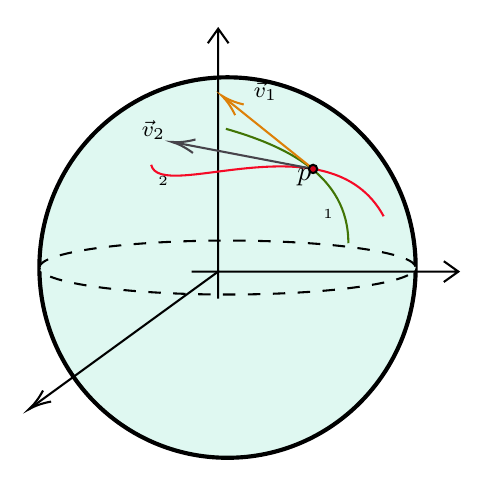
\begin{tikzpicture}[x=0.75pt,y=0.75pt,yscale=-1,xscale=1]
%uncomment if require: \path (0,256); %set diagram left start at 0, and has height of 256

%Shape: Ellipse [id:dp8621922183495604] 
\draw  [fill={rgb, 255:red, 223; green, 248; blue, 241 }  ,fill opacity=1 ][line width=1.5]  (205.14,135.71) .. controls (205.14,85.08) and (245.73,44.05) .. (295.79,44.05) .. controls (345.85,44.05) and (386.43,85.08) .. (386.43,135.71) .. controls (386.43,186.33) and (345.85,227.37) .. (295.79,227.37) .. controls (245.73,227.37) and (205.14,186.33) .. (205.14,135.71) -- cycle ;
%Shape: Ellipse [id:dp2859403935407516] 
\draw  [fill={rgb, 255:red, 223; green, 248; blue, 241 }  ,fill opacity=1 ][dash pattern={on 4.5pt off 4.5pt}] (205.14,135.71) .. controls (205.14,128.53) and (245.73,122.71) .. (295.79,122.71) .. controls (345.85,122.71) and (386.43,128.53) .. (386.43,135.71) .. controls (386.43,142.89) and (345.85,148.71) .. (295.79,148.71) .. controls (245.73,148.71) and (205.14,142.89) .. (205.14,135.71) -- cycle ;
%Shape: Axis 2D [id:dp5781161322417953] 
\draw  (278.43,137.66) -- (407,137.66)(291.29,20.64) -- (291.29,150.66) (400,132.66) -- (407,137.66) -- (400,142.66) (286.29,27.64) -- (291.29,20.64) -- (296.29,27.64)  ;
%Straight Lines [id:da986530720222472] 
\draw    (291.29,137.66) -- (201.62,202.87) ;
\draw [shift={(200,204.05)}, rotate = 323.97] [color={rgb, 255:red, 0; green, 0; blue, 0 }  ][line width=0.75]    (10.93,-3.29) .. controls (6.95,-1.4) and (3.31,-0.3) .. (0,0) .. controls (3.31,0.3) and (6.95,1.4) .. (10.93,3.29)   ;
%Curve Lines [id:da2567673398245671] 
\draw [color={rgb, 255:red, 245; green, 10; blue, 38 }  ,draw opacity=1 ]   (259,86.2) .. controls (263.29,105.12) and (345,63) .. (371,111) ;
%Curve Lines [id:da2661789837245453] 
\draw [color={rgb, 255:red, 65; green, 117; blue, 5 }  ,draw opacity=1 ]   (295,68.87) .. controls (323,76.87) and (354,90.87) .. (354,124) ;
%Straight Lines [id:da53165768173298] 
\draw [color={rgb, 255:red, 71; green, 68; blue, 75 }  ,draw opacity=1 ][fill={rgb, 255:red, 61; green, 57; blue, 57 }  ,fill opacity=1 ][line width=0.75]    (337,88.2) -- (270.96,75.58) ;
\draw [shift={(269,75.2)}, rotate = 10.82] [color={rgb, 255:red, 71; green, 68; blue, 75 }  ,draw opacity=1 ][line width=0.75]    (10.93,-3.29) .. controls (6.95,-1.4) and (3.31,-0.3) .. (0,0) .. controls (3.31,0.3) and (6.95,1.4) .. (10.93,3.29)   ;
%Straight Lines [id:da3674366892672871] 
\draw [color={rgb, 255:red, 221; green, 128; blue, 8 }  ,draw opacity=1 ][fill={rgb, 255:red, 61; green, 57; blue, 57 }  ,fill opacity=1 ][line width=0.75]    (337,88.2) -- (294.56,54.12) ;
\draw [shift={(293,52.87)}, rotate = 38.77] [color={rgb, 255:red, 221; green, 128; blue, 8 }  ,draw opacity=1 ][line width=0.75]    (10.93,-3.29) .. controls (6.95,-1.4) and (3.31,-0.3) .. (0,0) .. controls (3.31,0.3) and (6.95,1.4) .. (10.93,3.29)   ;
%Shape: Circle [id:dp7854098221379334] 
\draw  [fill={rgb, 255:red, 208; green, 2; blue, 27 }  ,fill opacity=1 ] (335,88.2) .. controls (335,87.1) and (335.9,86.2) .. (337,86.2) .. controls (338.1,86.2) and (339,87.1) .. (339,88.2) .. controls (339,89.3) and (338.1,90.2) .. (337,90.2) .. controls (335.9,90.2) and (335,89.3) .. (335,88.2) -- cycle ;

% Text Node
\draw (253,63.59) node [anchor=north west][inner sep=0.75pt]  [font=\footnotesize]  {$\vec{v}_{2}$};
% Text Node
\draw (340.43,106.05) node [anchor=north west][inner sep=0.75pt]  [font=\scriptsize]  {$\upsigma _{1} \ \ $};
% Text Node
\draw (261,90.6) node [anchor=north west][inner sep=0.75pt]  [font=\scriptsize]  {$\upsigma _{2} \ \ $};
% Text Node
\draw (307,44.59) node [anchor=north west][inner sep=0.75pt]  [font=\footnotesize]  {$\vec{v}_{1}$};
% Text Node
\draw (328,86.4) node [anchor=north west][inner sep=0.75pt]    {$p$};


\end{tikzpicture}

  \caption{Two tangent vectors and their representative curves are shown on the manifold at point $p$.}
\end{figure}
\noindent
In the above figure, we have two tangent vectors $\veb{v}_1$ and $\veb{v}_2$ at $p$ with $\sigma_1$ and $\sigma_2$ as their representative curves (that is, $\veb{v}_1 = [\sigma_1]$ and $\veb{v}_2 = [\sigma_2]$). We use a local chart $(U,\phi)$ around $p$ such that $\phi(p) = \veb{0} \in \mathbb{R}^m$.\\[0.3cm]
Consider the maps $\phi \circ \sigma_1$ and $\phi \circ \sigma_2$. Since a curve $\sigma$ maps an open interval to the manifold and the homeomorphism maps an open set in the manifold to an open set in $\mathbb{R}^m$, the above composite functions maps an open interval to an open set in $\mathbb{R}^m$.\\[0.3cm]
Now, the addition $\phi \circ \sigma_1 (t) + \phi \circ \sigma_2(t)$ is valid, since these are elements of $\mathbb{R}^m$ (actually, these are also curves in $\mathbb{R}^m$). Then we consider the map:
$$\phi^{-1}\circ (\phi \circ \sigma_1 (t) + \phi \circ \sigma_2(t))$$
which is a curve back on the manifold and passes through $p$ when $t=0$. We then define:
\begin{enumerate}
  \item $v_1+v_2 :=[\phi^{-1}\circ (\phi \circ \sigma_1  + \phi \circ \sigma_2)]$
  \item $rv :=[\phi^{-1}\circ (r\phi \circ \sigma )]\ \forall \ r\in \mathbb{R}$ 
\end{enumerate}
It can then be shown that these definitions are independent of the charts and the representative curves, and using these, the tangent space can be shown to be a vector space.
\subsubsection{Tangents as derivatives}
We saw a geometric way of defining tangents using the tangent space approach. Now, we will define it algebraically. The directional derivative of a function $f$ along a tangent  vector $v$ is defined as:
$$v(f) := \dv{t}f(\sigma(t))\Bigg|_{t=0}$$
where $v = [\sigma]$. This definition helps us to view $v$ as a differential operator on the space $C^\infty(\mathcal{M})$ of real-valued functions on the manifold. 
\begin{definition}[Derivations]
  A derivation at a point $p\in\mathcal{M}$ is a map $v_p:C^\infty(\mathcal{M})\rightarrow \mathbb{R}$ such that:
  \begin{itemize}
    \item 
    \begin{align*}
      v_p(f+g) &= v_p(f) + v_p(g) \ \forall \ f,g\in C^\infty(\mathcal{M})\\
      v_p(rf) &= r v_p(f) \ \forall \ f \in C^\infty(\mathcal{M}), r \in \mathbb{R}
    \end{align*}
    \item $v_p(fg) = f(p)v_p(g)+ g(p)v_p(f)\ \forall \ f,g\in C^\infty(\mathcal{M})$
  \end{itemize}
  The set of all derivations at $p$ is denoted as $D_p\mathcal{M}$
\end{definition}
The first condition tells us that $v$ should be a linear map and the second condition (kind of like the product rule) is the actual thing for which we call it \textit{derivation}. We can define:
\begin{align*}
  (v_1+v_2)(f) &:=v_1(f)+v_2(f) \ \forall v_1,v_2\in D_p\SM\\
(rv)(f) &:= rv(f)
\end{align*}
Also, note that:
\begin{align*}
  (v_1+v_2)(fg) &= v_1(fg) + v_2(fg) \\
  &= fv_1(g) + gv_1(f) + fv_2(g) + gv_2(f)\\
  &=f(v_1+v_2)(g) + g(v_1+v_2)(f)
\end{align*}
This gives a natural vector space structure to the space of derivations $D_p\SM$. Note that if we try to do the same analysis for $v_p\in D_p\SM$ and $w_q\in D_q\SM$, these $v_p+w_q$ will not satisfy the product rule and then will not be a valid vector. So, vectors at different point on a manifold cannot be added \emoji{face-with-rolling-eyes}\\[0.2cm] 
We can also show that $T_p\mathcal{M}$ and $D_p\mathcal{M}$ are actually \textit{isomorphic} and thus, both approaches can be taken to describe the tangent-space structure (However, the algebraic approach is a bit problematic for infinite-dimensional space). We shall henceforth use $T_p\SM$ and $D_p\SM$ as the same.
We now define a set of derivations of a function $f$ at $p$, with the help of a local chart $(U,\phi)$ where $f\in C^\infty$ and $\phi^\mu$ are the coordinate components.
$$\brac{\pdv{x^\mu}}_p f := \pdv{r^\mu}f\circ \phi^{-1}\Bigg|_{\phi(p)}\quad \mu = 1,2,\ldots, m$$
Note that in the right hand side, the partial derivative with respect to the coordinate is well defined, but in the left hand side, even though the notation is of partial derivative, the action is not well defined since the function is defined on the manifold which doesn't have the vector space structure required for definition of partial derivatives. Sometimes we use the notation $\pdv{f}{x^\mu}$ directly. Then, using this notation and also the fact that $\phi^{-1}\circ \phi(p) = p$, we can write:

$$\brac{\pdv{f}{x^\mu}} \brac{p} = \brac{\pdv{f}{x^\mu}}\brac{\phi^{-1}\circ \phi(p)} = \pdv{r^\mu}\brac{f\circ \phi^{-1}}{\phi(p)}$$
Then we can write 
$$\brac{\pdv{f}{x^\mu}}\circ \phi^{-1} \equiv   \pdv{r^\mu}\brac{f\circ \phi^{-1}}$$
\begin{ffact}
  Tangent vector acting on a constant function is zero, that is, $v_p(c) = 0$
\end{ffact}
\textit{Proof. } Suppose we have a constant real valued function $f\equiv c\in \re$. First, note that $v_p(1) = v_p(1\cdot 1) = 1v_p(1) + 1v_p(1) = 2v_p(1)\implies v_p(1)=0$. Then we will have $v_p(c) = v_p(c\cdot 1) = c v_p(1) = 0 $
\begin{proposition}
  Suppose $(U,\phi)$ is a chart with coordinates $x^i$. Then $\pdv{x^i}{x^j} = \tensor{\delta}{^i _j}$
\end{proposition}
\textit{Proof.} From the previous result, we have:
$$\pdv{x^i}{x^j}\brac{\phi(p)} = \pdv{x^i \circ x^{-1}}{r^j}\brac{\phi(p)} = \pdv{r^i\circ \phi \circ x^{-1}}{r^j}\brac{\phi(p)} =\pdv{r^i}{r^j}\brac{\phi(p)} = \tensor{\delta}{^i _j}$$
We just used the coordinate definition using the projection maps. \\[0.3cm]
These quantitites form a basis set for the vector space $D_p\mathcal{M}$. For that we have to check for linear independence and span of these quantitites. 
\begin{proposition}
 The set $\left\{\brac{\pdv{x^i}}_p \right\}$ is linearly independent.
\end{proposition}
\textit{Proof.}  $a^i \brac{\pdv{x^i}}_p = 0\implies  a^i \brac{\pdv{x^j}{x^i}}_p \implies a^i\tensor{\delta}{^j _i} = 0 \implies a^j = 0$
\begin{proposition}
  Every $v_p\in T_p\SM$ can be written as a linear combination of $\brac{\pdv{x^i}}_p$
\end{proposition}
\textit{Proof.} For the proof, we need to use the \text{Mean-Value Theorem}. For a continuously differentiable function $f:[a,b]\rightarrow \re$, $\exists \ c\in(a,b)$ such that $f'(c) = \frac{f(b)-f(a)}{b-a}\implies f(b) = f(a)+ f'(c)(b-a)$.\\[0.2cm] For a multi-variable function, let $U\subset \re^n$ be an open set and $H:U\rightarrow \re$ be a continuously differentiable function. Let $\veb{a},\veb{b}\in U$ and $l(\veb{a},\veb{b})\equiv \{(1-t)\veb{a}+t\veb{b}|t\in [0,1]\}\subset U$.\\[0.2cm] Then define $h:[0,1]\rightarrow \re$ such that $t\mapsto H((1-t)\veb{a}+t\veb{b}) = H(\veb{a}+t(\veb{b}-a))$.\\[0.2cm]
Note that $h(0) = H(\veb{a}), h(1) = H(\veb{b})$ and $h$ is continuously differentiable. Also,
$$h'(t) = \dv{t} H(\veb{a}+t(\veb{b}-\veb{a})) = (b^i - a^i)\pdv{H}{r^i}\Bigg|_{a+t(b-a)}$$
Now, we can apply the MVT for $\re$ on $h$ and we have for some $t_0\in (0,1)$:
\begin{align*}
  h(1) &= h(0) + (1-0)h'(t_0)\\
\implies H(b) &= H(a) +  (b^i - a^i)\pdv{H}{r^i}\Bigg|_{a+t_0(b-a)}
\end{align*}
Now, let us begin the actual proof. So let us take a chart $(U,\phi) on \SM$ and $f\in C^\infty(\SM)$. Then $f\circ\phi^{-1}: \phi(U)\rightarrow \re$ is a smooth map.\\[0.2cm]
Let $p\in U\implies \phi(p)\in \phi(U)$. As $\phi(U)$ is open subset of $\re^m$, there exists a $r>0$ such that $\SB(\phi(p), r)\subset \phi(U)$, from the basis definition of an open set. Then, let $q\in \phi^{-1}(\SB(\phi(p), r))$. Then $\phi(p)$ and $\phi(q)$ satisfy the condition $\{(1-t)\phi(p) +t\phi(q)|t\in[0,1]\}\subset \phi(U)$. Then we can apply the mean value theorem as seen before and we have:
\begin{align*}
  f(q)-f(p) &= f\circ\phi^{-1} \circ \phi(q) - f\circ\phi^{-1} \circ \phi(p)\\
&=f\circ\phi^{-1}(x^1(q), x^2(q),\ldots,x^m(q)) - f\circ\phi^{-1}(x^1(p), x^2(p),\ldots,x^m(p))\\
&=(x^i(q)-x^i(p))\pdv{f\circ\phi^{-1}}{r^i}\Bigg|_{\phi(p) +t(\phi(q)-\phi(p))}
\end{align*}
Now, if we fix $p$, then $$\pdv{f\circ\phi^{-1}}{r^i}\Bigg|_{\phi(p) +t(\phi(q)-\phi(p))}$$ depends only on $q$ and we denote it by $g_i(q)$. This implies that $g_i(p) = \pdv{f\circ\phi^{-1}}{r^i}\Bigg|_{\phi(p)} \equiv \brac{\pdv{x^i}}_p f$. We finally have:
$$f(q)=f(p)+(x^i(q)-x^i(p))g_i(q)\implies f\equiv f(p)+(x^i-x^i(p))g_i$$
Now let us apply some tangent vector $v_p$ to $f$. We have:
\begin{align*}
  v_p(f) &= v_p(f(p)+(x^i-x^i(p))g_i)\\
  &=\cancelto{0}{v_p(f(p))}+v_p((x^i-x^i(p))g_i) \quad (\because p \text{ fixed, $f(p)$ constant})\\
  &=v_p(g_i)\cancelto{0}{(x^i-x^i(p))_p} + v_p(x^i - x^i(p))g_i(p)\\
  &=(v_p(x^i) - v_p(x^i(p)))g_i(p)\\
  &=v_p(x^i)g_i(p) \\
  &= v_p(x^i)\brac{\pdv{x^i}}_p f
\end{align*}
Thus, we see that every tangent vector can be written as a combination of the set of derivations.\\[0.2cm]
So from the above two propositions, we proved that these quantities are indeed a basis for the tangent space. So any vector $v_p$ can be written as: $$v_p = c^i \brac{\pdv{x^i}}_p \implies v_p(x^j) = c^i \brac{\pdv{x^j}{x^i}}_p = c^i \tensor{\delta}{^j _i} = c^j \implies v_p = v_p(x^i) \brac{\pdv{x^i}}_p$$
We now define something which we had already seen earlier, the Jacobian. For that, let $\mathcal{M}$ and $\mathcal{N}$ be two manifolds and $(U,\phi)$ and $(V,\psi)$ be two charts on these manifolds respectively and $F: \mathcal{M}\rightarrow N$ be a smooth map between the manifolds such that $F(U) \subset V$. Let $F^i$ denote the $i^{\text{th}}$ component of $F$ in chart $(V,\psi)$. Then we have:
$$F^i := \psi^i \circ F = r^i \circ \psi \circ F$$
We call the matrix $[\pdv{F^i}{x^j}]$ to be the Jacobian matrix of $F$ relative to these charts and if the two manifolds have same dimension, we can also calculate the determinant of this matrix. If the manifolds are same and we have two overlapping charts, then the transition map $\gamma = \psi \circ \phi^{-1}$ is from $\mathbb{R}^m$ to $\mathbb{R}^m$. Previously, in the definition, we had $F:\mathcal{M}\rightarrow \mathcal{N}$. If we take $F= \gamma$, then $\mathcal{N},\mathcal{M} = \mathbb{R}^m$ whose coordinates are $r^\mu$. Then
$$\pdv{\gamma^i}{r^j}\brac{\phi(p)} = \pdv{\brac{\psi \circ \phi^{-1}}^i}{r^j}\brac{\phi(p)} =\pdv{r^i \circ \brac{\psi \circ \phi^{-1}}}{r^j}\brac{\phi(p)} = \pdv{ \psi^i { \circ \phi^{-1}}}{r^j}\brac{\phi(p)} = \pdv{\psi^i}{\phi^j}\brac{p}$$
What this tells us is that the Jacobian matrix of the transition map is the matrix of the partial derivatives at $p$. This is very similar to what we had earlier seen, the Jacobian written as $\pdv{x'}{x}$. 

\begin{theorem}[Inverse Function Theorem]
  \textbf{For $\mathbf{\mathbb{R}^n}$}: Let $F: W\rightarrow \mathbb{R}^n$ be a smooth map where $W$ is an open subset of $\mathbb{R}^n$. For $p\in W$, $F$ is locally invertible at $p$ iff determinant of the Jacobian matrix is not zero. \\[0.2cm]
  \textbf{For manifolds}: Let $F:\mathcal{M}\rightarrow \mathcal{N}$ be a smooth map between two manifolds and $p\in \mathcal{M}$. Let $(U,\phi)$ and $(V,\psi)$ be two charts about $p$ and $F(p)$ respectively and $F(U)\subset V$. Let $F^i = \psi^i \circ F$. Then $F$ is locally invertible at $p$ iff Jacobian determinant is non-zero.
\end{theorem}
This is a local result and hence, directly translated to manifolds too from $\mathbb{R}^n$.
\subsubsection{Push-forward (differential)}
Remember the pull-back? Huh, now this is its counterpart.\\[0.2cm]
Let $\SM$ and $\SN$ be two differentiable manifolds and $\psi: \SM\rightarrow \SN$ be a smooth map. The map $\psi$ induces a map between $T_p\SM$ and $T_{\psi(p)}\SN$ denoted by $\psi_{*p}$ or $d\psi_p$ which is called the differential of $\psi$ (basically, $p \mapsto \psi(p)$ under $\psi$ and the tangent plane at $p$ is mapped to tangent plane at $\psi(p)$) using this \textit{differential}. If $v_p\in T_p\SM$, then $\psi_{*p}(v_p)\in T_{\psi(p)}\SN$ and is defined by:
$$\psi_{*p}(v_p)(f) \equiv v_p(\psi^* f)\ \forall \ f\in \cty{\SN}$$
Let us now check that $\psi_{*p}(v_p)$ is indeed a member of the tangent plane at $\psi(p)$ in $N$. 
\begin{align*}
  \psi_{*p}(v_p)(c_1f_1 + c_2f_2) &= v_p(\psi^*(c_1f_1+c_2f_2))\\
  &=v_p(c_1(\psi^*f_1) + c_2(\psi^*f_2)) \qquad\quad \text{($\psi^*$ is a linear map)}\\
  &=c_1v_p(\psi^*f_1) + c_2 v_p(\psi^*f_2) \qquad\quad \text{($v_p$ is a linear map)}\\
  &=c_1 \psi_{*p}(v_p)(f_1)+c_2 \psi_{*p}(v_p)(f_2)
\end{align*}%
\begin{align*}
  \psi_{*p}(v_p)(fg) &= v_p(\psi^*(fg))\\
  &=v_p((\psi^*f)(\psi^*g))\\
  &=(\psi^*f)v_p(\psi^*g) +(\psi^*g)v_p(\psi^*f) \qquad\qquad \text{(Liebniz rule)}\\
  &= (\psi^*f)\psi_{*p}(v_p)(g) + (\psi^*g)\psi_{*p}(v_p)(f)
\end{align*}
Now, let us check that $\psi_{*p}$ is a linear map from $T_p\SM \rightarrow T_{\psi(p)}\SN$. For that, consider a linear combination of vectors from the tangent space of $\SM$. 
\begin{align*}
  \psi_{*p}(c_1 v_{p}+c_2 w_p)(f) &=(c_1 v_{p}+c_2 w_p)(\psi^* f)\\
&=c_1v_p(\psi^*f) + c_2w_p(\psi^*f)\\
&=c_1 \psi_{*p}(v_p)(f)+c_2 \psi_{*p}(w_p)(f)
\end{align*}
Thus, we proved the linearity of the push-forward. Now using this differential, we will obtain an expression which is analogous to the Jacobian seen earlier. For that, take charts $(U,\phi)$ and $(V,\chi)$ on $\SM$ and $\SN$ respectively, with coordinate functions $(x^1, x^2,\ldots, x^m)$ and $(y^1, y^2,\ldots, y^n)$ and $\psi: \SM\rightarrow \SN$ and consider $\psi_{*p}\brac{\pdv{x^i}}_p \in T_{\psi(p)}\SN$. 
\begin{align*}
  \psi_{*p}\brac{\pdv{x^i}}_p &=  \psi_{*p}\brac{\pdv{x^i}}_p\brac{y^j}\brac{\pdv{y^j}}_{\psi(p)}\quad\quad \text{(expanding with basis elements)}\\
  &=\brac{\pdv{x^i}}_p(\psi^* y^j)\brac{\pdv{y^j}}_{\psi(p)}\\
  &=\brac{\pdv{x^i}}_p(y^j\circ \psi)\brac{\pdv{y^j}}_{\psi(p)}\\
  &=\brac{\pdv{(y^j\circ \psi)}{x^i}}_p\brac{\pdv{y^j}}_{\psi(p)}
\end{align*}  
This looks very similar to the Jacobian thingy that we saw earlier and thus, push-forward is also kind of like the Jacobian matrix.\\[0.3cm]
\textbf{Pushing tangents to curves:}\\[0.2cm]
Let $\psi: \SM\rightarrow \SN$ and $\sigma: (a,b)\rightarrow \SM$ be a curve on $\SM$. Then $\psi\circ \sigma: (a,b)\rightarrow \SN$ is a curve on $\SN$. Then tangent vector $v$ to this curve at $(\psi\circ \sigma)(0)$ satisfies for any $f\in \cty{\SN}$: 
$$v(f) = \dv{t}f\circ (\psi\circ \sigma)\Bigg|_{t=0}$$
Now, these can be alternatively written as: 
$$v(f) = \dv{t} (\psi\circ \sigma)^* f\Bigg|_{t=0} = \dv{t}\sigma^*(f\circ \psi)\Bigg|_{t=0} =\dv{t}(f\circ \psi)\circ \sigma\Bigg|_{t=0} = w(f\circ\psi)$$
where $w$ is the tangent vector to the curve at $\sigma(0)$, acting on the function $f\circ\psi$ which can also be written as $w(\psi^*f)$. Using the definition of push-forward, this is nothing but $\psi_{*\sigma(0)}(w)(f)$\\
Now, since this is true for any smooth function $f$, we can write $v\equiv \psi_{*\sigma(0)}(w)$. In other words, the Jacobian of $\psi$ pushes the tangent vectors of $\sigma$ to tangent vectors of the image of $\sigma$ under $\psi$. 
\begin{figure}[H]
  \centering
  

\tikzset{every picture/.style={line width=0.75pt}} %set default line width to 0.75pt        

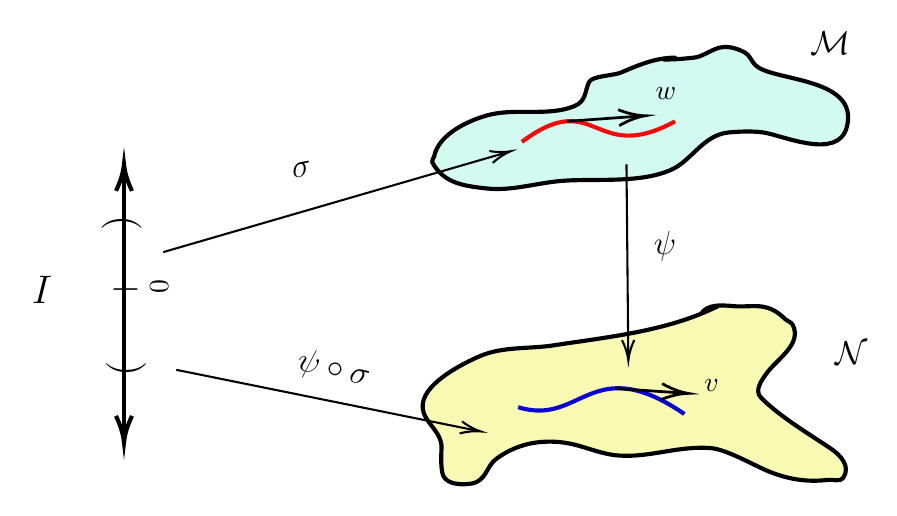
\begin{tikzpicture}[x=0.75pt,y=0.75pt,yscale=-1,xscale=1, scale=0.9]
%uncomment if require: \path (0,300); %set diagram left start at 0, and has height of 300

%Curve Lines [id:da9083608220761967] 
\draw [fill={rgb, 255:red, 130; green, 241; blue, 213 }  ,fill opacity=0.35 ][line width=1.5] [line join = round][line cap = round]   (419,36.9) .. controls (408.53,36.9) and (399.12,40.99) .. (390,44.9) .. controls (386.21,46.52) and (374.64,46.61) .. (373,49.9) .. controls (370.6,54.69) and (371.63,60.25) .. (365,62.9) .. controls (350.57,68.67) and (333.08,63.5) .. (318,67.9) .. controls (307.64,70.92) and (292.38,78) .. (290,89.9) .. controls (289.79,90.93) and (288.5,91.97) .. (289,92.9) .. controls (295.24,104.34) and (306.15,105.58) .. (318,106.9) .. controls (331.56,108.41) and (344.5,104.02) .. (358,102.9) .. controls (375.97,101.4) and (400.01,104.45) .. (417,96.9) .. controls (427.96,92.03) and (434.19,78.05) .. (448,76.9) .. controls (453.98,76.4) and (460.05,76.13) .. (466,76.9) .. controls (476.13,78.21) and (506.38,92.36) .. (511,73.9) .. controls (517.73,46.99) and (470.81,49.71) .. (462,40.9) .. controls (459.58,38.48) and (459.1,35.45) .. (456,33.9) .. controls (441.6,26.7) and (437.76,35.93) .. (429,36.9) .. controls (423.69,37.49) and (418.34,37.9) .. (413,37.9) ;
%Curve Lines [id:da9706399412764172] 
\draw [fill={rgb, 255:red, 243; green, 245; blue, 132 }  ,fill opacity=0.62 ][line width=1.5] [line join = round][line cap = round]   (442,169.9) .. controls (415.05,183.38) and (383.37,186.38) .. (354,190.9) .. controls (340.55,192.97) and (326.73,191.3) .. (314,196.9) .. controls (306.4,200.25) and (285.66,210.3) .. (284,221.9) .. controls (282.65,231.35) and (293.45,235.57) .. (294,244.9) .. controls (294.07,246.04) and (293.14,257.18) .. (295,260.9) .. controls (297.5,265.91) and (306.04,265.51) .. (310,264.9) .. controls (317.87,263.69) and (318.03,255.62) .. (323,251.9) .. controls (333.48,244.04) and (345.73,241.24) .. (359,242.9) .. controls (369.41,244.2) and (378.48,249.2) .. (389,249.9) .. controls (405.91,251.03) and (420.22,244.63) .. (438,245.9) .. controls (446.16,246.48) and (460.54,254.7) .. (468,257.9) .. controls (479.08,262.65) and (489.81,264.3) .. (501,262.9) .. controls (503.67,262.57) and (507.51,264.14) .. (509,261.9) .. controls (513.11,255.74) and (507.94,249.86) .. (502,245.9) .. controls (488.72,237.05) and (474.94,228.84) .. (465,218.9) .. controls (461.14,215.04) and (465.67,209.16) .. (468,205.9) .. controls (473.43,198.29) and (487.24,190.37) .. (482,179.9) .. controls (481.25,178.41) and (479.18,178.08) .. (478,176.9) .. controls (467.95,166.85) and (460.57,170.86) .. (450,169.9) .. controls (443.82,169.34) and (436.45,168.73) .. (433,173.9) ;
%Straight Lines [id:da7589756419214643] 
\draw [line width=1.5]    (124,97) -- (124,239.9) ;
\draw [shift={(124,242.9)}, rotate = 270] [color={rgb, 255:red, 0; green, 0; blue, 0 }  ][line width=1.5]    (14.21,-4.28) .. controls (9.04,-1.82) and (4.3,-0.39) .. (0,0) .. controls (4.3,0.39) and (9.04,1.82) .. (14.21,4.28)   ;
\draw [shift={(124,94)}, rotate = 90] [color={rgb, 255:red, 0; green, 0; blue, 0 }  ][line width=1.5]    (14.21,-4.28) .. controls (9.04,-1.82) and (4.3,-0.39) .. (0,0) .. controls (4.3,0.39) and (9.04,1.82) .. (14.21,4.28)   ;
%Straight Lines [id:da15285926618261458] 
\draw    (145,141) -- (329.08,87.56) ;
\draw [shift={(331,87)}, rotate = 163.81] [color={rgb, 255:red, 0; green, 0; blue, 0 }  ][line width=0.75]    (10.93,-3.29) .. controls (6.95,-1.4) and (3.31,-0.3) .. (0,0) .. controls (3.31,0.3) and (6.95,1.4) .. (10.93,3.29)   ;
%Straight Lines [id:da4966374031544514] 
\draw    (152,204) -- (313.04,236.6) ;
\draw [shift={(315,237)}, rotate = 191.45] [color={rgb, 255:red, 0; green, 0; blue, 0 }  ][line width=0.75]    (10.93,-3.29) .. controls (6.95,-1.4) and (3.31,-0.3) .. (0,0) .. controls (3.31,0.3) and (6.95,1.4) .. (10.93,3.29)   ;
%Curve Lines [id:da714564075847796] 
\draw [color={rgb, 255:red, 245; green, 9; blue, 9 }  ,draw opacity=1 ][line width=1.5]    (337,82) .. controls (377,52) and (375,95) .. (419,71) ;
%Curve Lines [id:da26538820278083086] 
\draw [color={rgb, 255:red, 9; green, 5; blue, 211 }  ,draw opacity=1 ][line width=1.5]    (335,224) .. controls (369,234.62) and (374,193.62) .. (424,227.62) ;
%Straight Lines [id:da20362367095818434] 
\draw    (393,94) -- (393.98,197) ;
\draw [shift={(394,199)}, rotate = 269.45] [color={rgb, 255:red, 0; green, 0; blue, 0 }  ][line width=0.75]    (10.93,-3.29) .. controls (6.95,-1.4) and (3.31,-0.3) .. (0,0) .. controls (3.31,0.3) and (6.95,1.4) .. (10.93,3.29)   ;
%Straight Lines [id:da09726797419252065] 
\draw [line width=1.0]    (361,71) -- (400.01,68.21) ;
\draw [shift={(403,68)}, rotate = 175.91] [color={rgb, 255:red, 0; green, 0; blue, 0 }  ][line width=1.0]    (14.21,-4.28) .. controls (9.04,-1.82) and (4.3,-0.39) .. (0,0) .. controls (4.3,0.39) and (9.04,1.82) .. (14.21,4.28)   ;
%Straight Lines [id:da4554197621882127] 
\draw [line width=1.0]    (387,214) -- (423.01,216.42) ;
\draw [shift={(426,216.62)}, rotate = 183.84] [color={rgb, 255:red, 0; green, 0; blue, 0 }  ][line width=1.0]    (14.21,-4.28) .. controls (9.04,-1.82) and (4.3,-0.39) .. (0,0) .. controls (4.3,0.39) and (9.04,1.82) .. (14.21,4.28)   ;

% Text Node
\draw (135.1,119.5) node [anchor=north west][inner sep=0.75pt]  [font=\Large,rotate=-90]  {$($};
% Text Node
\draw (112.9,209.5) node [anchor=north west][inner sep=0.75pt]  [font=\Large,rotate=-270]  {$($};
% Text Node
\draw (115,152.4) node [anchor=north west][inner sep=0.75pt]  [font=\Large]  {$-$};
% Text Node
\draw (136.4,165) node [anchor=north west][inner sep=0.75pt]  [font=\normalsize,rotate=-270]  {$0$};
% Text Node
\draw (73,152.4) node [anchor=north west][inner sep=0.75pt]  [font=\Large]  {$I$};
% Text Node
\draw (490,21.4) node [anchor=north west][inner sep=0.75pt]  [font=\large]  {$\mathcal{M}$};
% Text Node
\draw (503,187.4) node [anchor=north west][inner sep=0.75pt]  [font=\large]  {$\mathcal{N}$};
% Text Node
\draw (406,128.4) node [anchor=north west][inner sep=0.75pt]  [font=\large]  {$\psi $};
% Text Node
\draw (211.36,92.75) node [anchor=north west][inner sep=0.75pt]  [font=\large,rotate=-349.5]  {$\sigma $};
% Text Node
\draw (217.82,189.56) node [anchor=north west][inner sep=0.75pt]  [font=\large,rotate=-13.4]  {$\psi \circ \sigma $};
% Text Node
\draw (433,207.4) node [anchor=north west][inner sep=0.75pt]    {$v$};
% Text Node
\draw (407,51.4) node [anchor=north west][inner sep=0.75pt]    {$w$};


\end{tikzpicture}

  \caption{Diagram showing the pushing-forward of tangent to curves in different manifolds.}
\end{figure}
\subsubsection{Tangent Bundles}
The tangent bundle of a manifold $\mathcal{M}$ is the union of all the tangent spaces, hence: 
$$T\mathcal{M} = \bigcup\limits_{p\in \mathcal{M}}T_p\mathcal{M}$$
We can define a `natural' (coordinate or chart independent) map $\pi$ from the tangent bundle to the manifold given by $\pi(v) = p, \ \ v \in T_p\mathcal{M}$ (since tangent bundle is the union of tangent spaces, it indeed consists of elements from $\{T_p\SM\}$). The map $\pi$ is sometimes called the \textit{canonical projection}.
Notice that the tangent bundle is just a set, with no structure or anything else. Let us modify this a bit. Suppose we have a chart $(U,\phi)$, then we will have:
$$TU =  \bigcup\limits_{p\in {U}}T_p{U}= \bigcup\limits_{p\in \mathcal{U}}T_p\mathcal{M}$$ 
The last two things can be shown to be equal. Since the set of derivations form a basis for the tangent space at $p$, we can write the tangent vector uniquely as a linear combination:
$$T_p\mathcal{M}\ni v_p = \sum\limits_{i}^n \dot{q}^i(v_p) \pdv{x^i}\Bigg|_p$$
Here, $\dot{q}^i: \pi^{-1}(U)\rightarrow \mathbb{R}$ are $n$ real-valued functions \footnote{The notation is borrowed from Lagrangian formulation of classical mechanics, where the manifold becomes the configuration space of the mechanical system}. Let us also define $q^i:\pi^{-1}(U)\rightarrow \re, {q}^i\equiv x^i\circ \pi = \pi^*x^i$ and $\bar{phi}:\phi^{-1}(U)\rightarrow \re^{2n}$
$$\bar{\phi}(v_p)\equiv \brac{q^1(v_p), q^2(v_p),\ldots,q^n(v_p),\dot{q}^1(v_p), \dot{q}^2(v_p),\ldots,\dot{q}^n(v_p)}$$ 
Note that $\bar{\phi}$ has an inverse such that $\brac{q^1(v_p), q^2(v_p),\ldots,q^n(v_p),\dot{q}^1(v_p), \dot{q}^2(v_p),\ldots,\dot{q}^n(v_p)} \mapsto \sum\limits_{i}^n \dot{q}^i(v_p) \pdv{x^i}\Bigg|_p$ and is thus a bijection. Also, 
\begin{align*}
  q^i(v_p) &= x^i\circ\pi(v_p) = x^i(p)\\
  v_p &= \dot{q}^i(v_p) \pdv{x^i}\Bigg|_p \implies  \dot{q}^i(v_p) = v_p[x^i]
\end{align*}
Thus, the function $\bar{\phi}$ becomes:
$$\bar{\phi}(v_p)\equiv \brac{x^1(p), x^2(p),\ldots,x^n(p),v_p[x^1], v_p[x^2],\ldots,v_p[x^n]}$$ 
\begin{figure}[H]
  \centering 
  

\tikzset{every picture/.style={line width=0.75pt}} %set default line width to 0.75pt        

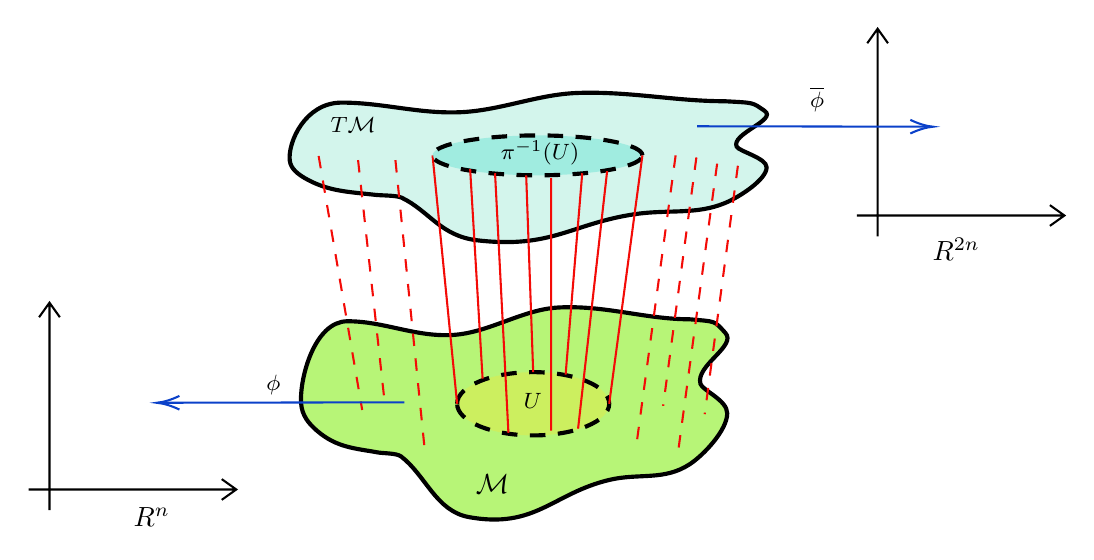
\begin{tikzpicture}[x=0.75pt,y=0.75pt,yscale=-1,xscale=1]
%uncomment if require: \path (0,351); %set diagram left start at 0, and has height of 351

%Shape: Boxed Bezier Curve [id:dp7555542346097139] 
\draw [fill={rgb, 255:red, 211; green, 245; blue, 236 }  ,fill opacity=1 ][line width=1.5]    (391.34,61.94) .. controls (367.37,61.94) and (345.22,57.03) .. (320.2,57.96) .. controls (300.91,58.67) and (282.94,66.54) .. (263.47,67.25) .. controls (243.27,67.98) and (226.53,62.6) .. (206.75,62.6) .. controls (189.05,62.6) and (180.8,81.91) .. (181.76,90.47) .. controls (182.21,94.49) and (185.77,97.27) .. (190.41,99.76) .. controls (201.06,105.48) and (210.83,105.65) .. (223.1,107.06) .. controls (225.93,107.38) and (233.27,107.27) .. (235.59,108.38) .. controls (248.94,114.76) and (254.4,126.91) .. (272.13,128.95) .. controls (308.22,133.11) and (317.45,120.88) .. (348.08,116.35) .. controls (363.96,114) and (377.58,116.74) .. (391.34,111.04) .. controls (398.74,107.97) and (411.53,99.55) .. (411.53,93.79) .. controls (411.53,89.32) and (398.16,86.03) .. (397.11,83.84) .. controls (394.13,77.68) and (416.9,70.96) .. (410.56,66.58) .. controls (404.35,62.3) and (405.76,62.75) .. (391.34,61.94) -- cycle ;
%Shape: Boxed Bezier Curve [id:dp6883735068899058] 
\draw [fill={rgb, 255:red, 158; green, 241; blue, 71 }  ,fill opacity=0.74 ][line width=1.5]    (374.5,167) .. controls (353.09,167) and (333.29,160.03) .. (310.94,161.34) .. controls (293.71,162.35) and (277.65,173.54) .. (260.26,174.55) .. controls (242.2,175.59) and (227.24,167.94) .. (209.57,167.94) .. controls (193.76,167.94) and (186.39,195.39) .. (187.24,207.57) .. controls (187.64,213.29) and (190.83,217.23) .. (194.97,220.77) .. controls (204.49,228.9) and (213.22,229.14) .. (224.18,231.15) .. controls (226.71,231.61) and (233.27,231.46) .. (235.34,233.04) .. controls (247.26,242.1) and (252.15,259.38) .. (267.99,262.28) .. controls (300.24,268.18) and (308.48,250.8) .. (335.85,244.36) .. controls (350.04,241.02) and (362.21,244.91) .. (374.5,236.81) .. controls (381.12,232.45) and (392.54,220.47) .. (392.54,212.28) .. controls (392.54,205.93) and (380.6,201.25) .. (379.66,198.13) .. controls (377,189.38) and (397.34,179.82) .. (391.68,173.6) .. controls (386.13,167.51) and (387.39,168.15) .. (374.5,167) -- cycle ;
%Shape: Ellipse [id:dp7913055919056734] 
\draw  [fill={rgb, 255:red, 245; green, 230; blue, 53 }  ,fill opacity=0.35 ][dash pattern={on 5.63pt off 4.5pt}][line width=1.5]  (262.41,207.7) .. controls (262.41,199.28) and (278.81,192.46) .. (299.05,192.46) .. controls (319.28,192.46) and (335.68,199.28) .. (335.68,207.7) .. controls (335.68,216.12) and (319.28,222.95) .. (299.05,222.95) .. controls (278.81,222.95) and (262.41,216.12) .. (262.41,207.7) -- cycle ;
%Straight Lines [id:da38840826454836663] 
\draw [color={rgb, 255:red, 243; green, 11; blue, 7 }  ,draw opacity=1 ][line width=0.75]    (250.56,88.02) -- (262.41,207.7) ;
%Shape: Ellipse [id:dp3372595327826894] 
\draw  [fill={rgb, 255:red, 119; green, 230; blue, 215 }  ,fill opacity=0.55 ][dash pattern={on 5.63pt off 4.5pt}][line width=1.5]  (351.68,88.02) .. controls (351.68,82.72) and (329.05,78.41) .. (301.12,78.41) .. controls (273.2,78.41) and (250.56,82.72) .. (250.56,88.02) .. controls (250.56,93.33) and (273.2,97.63) .. (301.12,97.63) .. controls (329.05,97.63) and (351.68,93.33) .. (351.68,88.02) -- cycle ;
%Straight Lines [id:da561591323588785] 
\draw [color={rgb, 255:red, 243; green, 11; blue, 7 }  ,draw opacity=1 ][line width=0.75]    (351.68,88.02) -- (335.68,207.7) ;
%Straight Lines [id:da690868976884767] 
\draw [color={rgb, 255:red, 243; green, 11; blue, 7 }  ,draw opacity=1 ][line width=0.75]    (334.68,95.63) -- (320.68,219.7) ;
%Straight Lines [id:da0643786859358153] 
\draw [color={rgb, 255:red, 243; green, 11; blue, 7 }  ,draw opacity=1 ][line width=0.75]    (280.68,96.63) -- (287.12,221.7) ;
%Straight Lines [id:da5276401921204039] 
\draw [color={rgb, 255:red, 243; green, 11; blue, 7 }  ,draw opacity=1 ][line width=0.75]    (307.72,98.81) -- (307.68,220.63) ;
%Straight Lines [id:da02591874235055658] 
\draw [color={rgb, 255:red, 243; green, 11; blue, 7 }  ,draw opacity=1 ][line width=0.75]    (268.68,94.63) -- (274.68,195.63) ;
%Straight Lines [id:da13234226839924923] 
\draw [color={rgb, 255:red, 243; green, 11; blue, 7 }  ,draw opacity=1 ][line width=0.75]    (295.68,97.63) -- (299.05,192.46) ;
%Straight Lines [id:da10881113373921192] 
\draw [color={rgb, 255:red, 243; green, 11; blue, 7 }  ,draw opacity=1 ][line width=0.75]    (322.68,96.63) -- (314.68,193.63) ;
%Straight Lines [id:da1622212363017358] 
\draw [color={rgb, 255:red, 243; green, 11; blue, 7 }  ,draw opacity=1 ][line width=0.75]  [dash pattern={on 4.5pt off 4.5pt}]  (367.68,88.02) -- (348.68,228.3) ;
%Straight Lines [id:da48330270456949853] 
\draw [color={rgb, 255:red, 243; green, 11; blue, 7 }  ,draw opacity=1 ][line width=0.75]  [dash pattern={on 4.5pt off 4.5pt}]  (377.68,89.02) -- (361.68,208.7) ;
%Straight Lines [id:da2990883543810654] 
\draw [color={rgb, 255:red, 243; green, 11; blue, 7 }  ,draw opacity=1 ][line width=0.75]  [dash pattern={on 4.5pt off 4.5pt}]  (195.68,88.3) -- (216.68,210.7) ;
%Straight Lines [id:da95060641908313] 
\draw [color={rgb, 255:red, 243; green, 11; blue, 7 }  ,draw opacity=1 ][line width=0.75]  [dash pattern={on 4.5pt off 4.5pt}]  (214.68,90.3) -- (227.68,208.7) ;
%Straight Lines [id:da7748858791112593] 
\draw [color={rgb, 255:red, 243; green, 11; blue, 7 }  ,draw opacity=1 ][line width=0.75]  [dash pattern={on 4.5pt off 4.5pt}]  (232.68,90.3) -- (246.68,228.7) ;
%Straight Lines [id:da23543355149656475] 
\draw [color={rgb, 255:red, 243; green, 11; blue, 7 }  ,draw opacity=1 ][line width=0.75]  [dash pattern={on 4.5pt off 4.5pt}]  (387.68,92.02) -- (368.68,232.3) ;
%Straight Lines [id:da252934263423064] 
\draw [color={rgb, 255:red, 243; green, 11; blue, 7 }  ,draw opacity=1 ][line width=0.75]  [dash pattern={on 4.5pt off 4.5pt}]  (397.68,93.02) -- (381.68,212.7) ;
%Shape: Axis 2D [id:dp028583688594270185] 
\draw  (56,249) -- (156,249)(66,159) -- (66,259) (149,244) -- (156,249) -- (149,254) (61,166) -- (66,159) -- (71,166)  ;
%Shape: Axis 2D [id:dp8970413200540654] 
\draw  (455,117) -- (555,117)(465,27) -- (465,127) (548,112) -- (555,117) -- (548,122) (460,34) -- (465,27) -- (470,34)  ;
%Straight Lines [id:da828009539651172] 
\draw [color={rgb, 255:red, 11; green, 65; blue, 201 }  ,draw opacity=1 ]   (237,207) -- (119.68,207.21) ;
\draw [shift={(117.68,207.22)}, rotate = 359.9] [color={rgb, 255:red, 11; green, 65; blue, 201 }  ,draw opacity=1 ][line width=0.75]    (10.93,-3.29) .. controls (6.95,-1.4) and (3.31,-0.3) .. (0,0) .. controls (3.31,0.3) and (6.95,1.4) .. (10.93,3.29)   ;
%Straight Lines [id:da45797751736499215] 
\draw [color={rgb, 255:red, 11; green, 65; blue, 201 }  ,draw opacity=1 ]   (378,74) -- (489.68,74.21) ;
\draw [shift={(491.68,74.22)}, rotate = 180.11] [color={rgb, 255:red, 11; green, 65; blue, 201 }  ,draw opacity=1 ][line width=0.75]    (10.93,-3.29) .. controls (6.95,-1.4) and (3.31,-0.3) .. (0,0) .. controls (3.31,0.3) and (6.95,1.4) .. (10.93,3.29)   ;

% Text Node
\draw (270,240.4) node [anchor=north west][inner sep=0.75pt]    {$\mathcal{M}$};
% Text Node
\draw (282,79.4) node [anchor=north west][inner sep=0.75pt]  [font=\footnotesize]  {$\pi ^{-1}( U)$};
% Text Node
\draw (293,201.4) node [anchor=north west][inner sep=0.75pt]  [font=\footnotesize]  {$U$};
% Text Node
\draw (200,68.4) node [anchor=north west][inner sep=0.75pt]  [font=\footnotesize]  {$T\mathcal{M}$};
% Text Node
\draw (105,256.4) node [anchor=north west][inner sep=0.75pt]    {$\mathbb{R}^{n}$};
% Text Node
\draw (490,126.4) node [anchor=north west][inner sep=0.75pt]    {$\mathbb{R}^{2n}$};
% Text Node
\draw (169,192.4) node [anchor=north west][inner sep=0.75pt]  [font=\footnotesize]  {$\phi $};
% Text Node
\draw (431,53.4) node [anchor=north west][inner sep=0.75pt]  [font=\footnotesize]  {$\overline{\phi }$};


\end{tikzpicture}

  \caption{Diagram showing the chart $\brac{\pi^{-1}(U),\bar{\phi}}$. The red lines represent the tangent space at each point of the manifold. Solid lines represent the tangent spaces for points belonging in $U$}
\end{figure}
\begin{lemma}
  The pair $\brac{\pi^{-1}(U),\bar{\phi}}$ is a chart on $T\SM$, often called the \textit{bundle chart}.
\end{lemma}
% \textit{Proof.} To prove that it is indeed a chart, we need to check if there exists a homeomorphism between the open sets $\pi^{-1}(U)$ and $\bar{\phi}(\pi^{-1}(U))$.\\[0.2cm] Firstly, note that $\bar{\phi}(\pi^{-1}(U)) = \phi(U)\times \re^n$. To understand this, observe that $\bar{\phi}$ acts on a tangent vector $v_p$, giving a $2n$ component vector, whose first $n$ components $\{q^i(v_p)\}$ are simply the coordinates of point $p$ (since $\pi$ takes $v_p$ to $p$) and hence these belong to $\phi(U)$. The last $n$ components can be arbitrary real numbers and hence belong to $\re^n$. Now, since $\re^n$ and $\phi(U)$ both are open sets, $\phi(U)\times \re^n$ is also open.  \\[0.2cm]
% Now, let us check if $\bar{\phi}$ is a homeomorphism. The components of $\bar{\phi}$ are smooth maps and hence $\bar{\phi}$ is smooth, hence continuous. \textcolor{red}{PROOF LEFT!}
The tangent bundle can also be shown to be \textit{Hausdorff} and \textit{second countable}. Well, tangent bundles are a special case of something called a fibre bundle. 
\begin{figure}[H]
  \centering 
  

\tikzset{every picture/.style={line width=0.75pt}} %set default line width to 0.75pt        

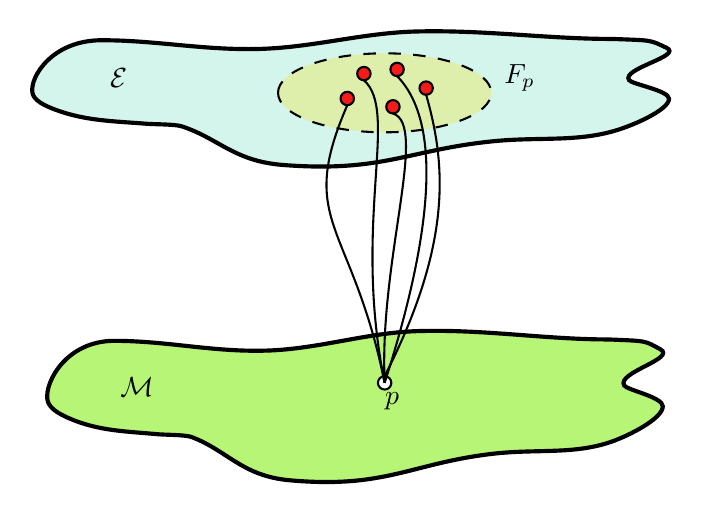
\begin{tikzpicture}[x=0.75pt,y=0.75pt,yscale=-1,xscale=1]
%uncomment if require: \path (0,351); %set diagram left start at 0, and has height of 351

%Shape: Boxed Bezier Curve [id:dp1046279221987515] 
\draw [fill={rgb, 255:red, 211; green, 245; blue, 236 }  ,fill opacity=1 ][line width=1.5]    (437.84,58.55) .. controls (405.85,58.55) and (376.27,54.11) .. (342.87,54.95) .. controls (317.13,55.59) and (293.14,62.72) .. (267.15,63.36) .. controls (240.17,64.03) and (217.83,59.16) .. (191.43,59.16) .. controls (167.8,59.16) and (156.79,76.64) .. (158.06,84.39) .. controls (158.66,88.04) and (163.42,90.55) .. (169.61,92.81) .. controls (183.83,97.99) and (196.88,98.14) .. (213.25,99.42) .. controls (217.04,99.71) and (226.83,99.61) .. (229.93,100.62) .. controls (247.74,106.39) and (255.04,117.4) .. (278.7,119.25) .. controls (326.89,123.01) and (339.2,111.93) .. (380.09,107.83) .. controls (401.29,105.7) and (419.47,108.19) .. (437.84,103.02) .. controls (447.73,100.25) and (464.79,92.62) .. (464.79,87.4) .. controls (464.79,83.35) and (446.95,80.37) .. (445.54,78.39) .. controls (441.57,72.81) and (471.96,66.72) .. (463.51,62.76) .. controls (455.21,58.88) and (457.09,59.29) .. (437.84,58.55) -- cycle ;
%Shape: Ellipse [id:dp7051113917362648] 
\draw  [fill={rgb, 255:red, 245; green, 230; blue, 53 }  ,fill opacity=0.35 ][dash pattern={on 4.5pt off 4.5pt}] (276.41,84.49) .. controls (276.41,73.98) and (299.41,65.46) .. (327.78,65.46) .. controls (356.14,65.46) and (379.14,73.98) .. (379.14,84.49) .. controls (379.14,95) and (356.14,103.52) .. (327.78,103.52) .. controls (299.41,103.52) and (276.41,95) .. (276.41,84.49) -- cycle ;
%Shape: Boxed Bezier Curve [id:dp6248237388540854] 
\draw [fill={rgb, 255:red, 158; green, 241; blue, 71 }  ,fill opacity=0.74 ][line width=1.5]    (435.74,203.32) .. controls (404.82,203.32) and (376.22,198.36) .. (343.93,199.29) .. controls (319.05,200.01) and (295.86,207.98) .. (270.73,208.7) .. controls (244.65,209.44) and (223.04,203.99) .. (197.53,203.99) .. controls (174.68,203.99) and (164.04,223.54) .. (165.27,232.2) .. controls (165.85,236.28) and (170.45,239.09) .. (176.44,241.61) .. controls (190.18,247.39) and (202.79,247.57) .. (218.62,249) .. controls (222.28,249.33) and (231.75,249.21) .. (234.75,250.34) .. controls (251.96,256.79) and (259.02,269.1) .. (281.89,271.16) .. controls (328.48,275.36) and (340.38,262.98) .. (379.91,258.4) .. controls (400.41,256.02) and (417.98,258.79) .. (435.74,253.03) .. controls (445.3,249.92) and (461.8,241.4) .. (461.8,235.56) .. controls (461.8,231.04) and (444.55,227.71) .. (443.19,225.49) .. controls (439.35,219.26) and (468.73,212.45) .. (460.56,208.02) .. controls (452.54,203.68) and (454.35,204.14) .. (435.74,203.32) -- cycle ;
%Shape: Circle [id:dp6027797339068129] 
\draw  [fill={rgb, 255:red, 255; green, 255; blue, 255 }  ,fill opacity=1 ] (324.55,224.22) .. controls (324.55,222.44) and (325.99,221) .. (327.78,221) .. controls (329.56,221) and (331,222.44) .. (331,224.22) .. controls (331,226.01) and (329.56,227.45) .. (327.78,227.45) .. controls (325.99,227.45) and (324.55,226.01) .. (324.55,224.22) -- cycle ;
%Shape: Circle [id:dp7978124382575595] 
\draw  [fill={rgb, 255:red, 245; green, 27; blue, 27 }  ,fill opacity=1 ] (314.55,75.22) .. controls (314.55,73.44) and (315.99,72) .. (317.78,72) .. controls (319.56,72) and (321,73.44) .. (321,75.22) .. controls (321,77.01) and (319.56,78.45) .. (317.78,78.45) .. controls (315.99,78.45) and (314.55,77.01) .. (314.55,75.22) -- cycle ;
%Shape: Circle [id:dp2405724773178366] 
\draw  [fill={rgb, 255:red, 245; green, 27; blue, 27 }  ,fill opacity=1 ] (328.55,91.22) .. controls (328.55,89.44) and (329.99,88) .. (331.78,88) .. controls (333.56,88) and (335,89.44) .. (335,91.22) .. controls (335,93.01) and (333.56,94.45) .. (331.78,94.45) .. controls (329.99,94.45) and (328.55,93.01) .. (328.55,91.22) -- cycle ;
%Shape: Circle [id:dp15559748198633383] 
\draw  [fill={rgb, 255:red, 245; green, 27; blue, 27 }  ,fill opacity=1 ] (330.55,73.22) .. controls (330.55,71.44) and (331.99,70) .. (333.78,70) .. controls (335.56,70) and (337,71.44) .. (337,73.22) .. controls (337,75.01) and (335.56,76.45) .. (333.78,76.45) .. controls (331.99,76.45) and (330.55,75.01) .. (330.55,73.22) -- cycle ;
%Shape: Circle [id:dp9974828834451859] 
\draw  [fill={rgb, 255:red, 245; green, 27; blue, 27 }  ,fill opacity=1 ] (344.55,82.22) .. controls (344.55,80.44) and (345.99,79) .. (347.78,79) .. controls (349.56,79) and (351,80.44) .. (351,82.22) .. controls (351,84.01) and (349.56,85.45) .. (347.78,85.45) .. controls (345.99,85.45) and (344.55,84.01) .. (344.55,82.22) -- cycle ;
%Shape: Circle [id:dp7618982493592206] 
\draw  [fill={rgb, 255:red, 245; green, 27; blue, 27 }  ,fill opacity=1 ] (306.55,87.22) .. controls (306.55,85.44) and (307.99,84) .. (309.78,84) .. controls (311.56,84) and (313,85.44) .. (313,87.22) .. controls (313,89.01) and (311.56,90.45) .. (309.78,90.45) .. controls (307.99,90.45) and (306.55,89.01) .. (306.55,87.22) -- cycle ;
%Curve Lines [id:da05883862390293093] 
\draw    (309.78,90.45) .. controls (285,147.53) and (312,146.53) .. (327.78,224.22) ;
%Curve Lines [id:da18762006209771054] 
\draw    (317.78,78.45) .. controls (335,93.53) and (312,146.53) .. (327.78,224.22) ;
%Curve Lines [id:da37581019078658384] 
\draw    (333.78,76.45) .. controls (355,98.18) and (351.78,149.18) .. (327.78,224.22) ;
%Curve Lines [id:da19009776774897946] 
\draw    (347.78,85.45) .. controls (357,117.9) and (361,155.9) .. (327.78,221) ;
%Curve Lines [id:da2576706771011591] 
\draw    (331.78,94.45) .. controls (349,99.9) and (325,164.9) .. (327.78,224.22) ;

% Text Node
\draw (194,71.4) node [anchor=north west][inner sep=0.75pt]    {$\mathcal{E}$};
% Text Node
\draw (199,220.4) node [anchor=north west][inner sep=0.75pt]    {$\mathcal{M}$};
% Text Node
\draw (326.55,227.62) node [anchor=north west][inner sep=0.75pt]    {$p$};
% Text Node
\draw (384,69.4) node [anchor=north west][inner sep=0.75pt]    {$F_{p}$};


\end{tikzpicture}

  \caption{Diagram showing the base space, total space and the fibre of a point $p$}
\end{figure}
\begin{definition}[Bundle]
  Given a map $\pi: \mathcal{E}\rightarrow M$, the inverse image $pi^{-1}(p)$ to be the \textit{fibre} at $p\in \mathcal{M}$, denoted as $E_p$. For two maps $\pi: \mathcal{E}\rightarrow M$ and $\pi: \mathcal{E}'\rightarrow M$, a map $\phi$ is said to be fibre-preserving if $\phi(E_p)\subset E_p'$.\\[0.2cm]
  A bundle is a triple $(\mathcal{E},\mathcal{M},\pi)$ consisting of manifolds $\mathcal{M}$ which is called the \textit{base space} and the manifold $\mathcal{E}$, called the \textit{total space} and $\pi$ is a continuous, surjective map from the total space to the base space.  
\end{definition}

\begin{figure}[H]
  \centering 
  

% Pattern Info
 
\tikzset{
pattern size/.store in=\mcSize, 
pattern size = 5pt,
pattern thickness/.store in=\mcThickness, 
pattern thickness = 0.3pt,
pattern radius/.store in=\mcRadius, 
pattern radius = 1pt}
\makeatletter
\pgfutil@ifundefined{pgf@pattern@name@_n2wu1tgz5}{
\pgfdeclarepatternformonly[\mcThickness,\mcSize]{_n2wu1tgz5}
{\pgfqpoint{0pt}{0pt}}
{\pgfpoint{\mcSize+\mcThickness}{\mcSize+\mcThickness}}
{\pgfpoint{\mcSize}{\mcSize}}
{
\pgfsetcolor{\tikz@pattern@color}
\pgfsetlinewidth{\mcThickness}
\pgfpathmoveto{\pgfqpoint{0pt}{0pt}}
\pgfpathlineto{\pgfpoint{\mcSize+\mcThickness}{\mcSize+\mcThickness}}
\pgfusepath{stroke}
}}
\makeatother
\tikzset{every picture/.style={line width=0.75pt}} %set default line width to 0.75pt        

\begin{tikzpicture}[x=0.75pt,y=0.75pt,yscale=-1,xscale=1]
%uncomment if require: \path (0,351); %set diagram left start at 0, and has height of 351

%Shape: Boxed Bezier Curve [id:dp12157575364814821] 
\draw [fill={rgb, 255:red, 171; green, 85; blue, 240 }  ,fill opacity=0.37 ][line width=1.5]    (370.11,211.58) .. controls (350.57,211.58) and (332.5,205.11) .. (312.1,206.33) .. controls (296.38,207.27) and (281.73,217.64) .. (265.86,218.57) .. controls (249.38,219.54) and (235.73,212.45) .. (219.61,212.45) .. controls (205.18,212.45) and (198.46,237.89) .. (199.23,249.18) .. controls (199.6,254.48) and (202.51,258.14) .. (206.29,261.42) .. controls (214.97,268.96) and (222.94,269.18) .. (232.94,271.04) .. controls (235.25,271.47) and (241.23,271.33) .. (243.13,272.79) .. controls (254,281.19) and (258.46,297.21) .. (272.91,299.9) .. controls (302.34,305.37) and (309.86,289.25) .. (334.84,283.29) .. controls (347.79,280.19) and (358.89,283.8) .. (370.11,276.29) .. controls (376.15,272.25) and (386.57,261.15) .. (386.57,253.55) .. controls (386.57,247.67) and (375.67,243.32) .. (374.81,240.43) .. controls (372.39,232.32) and (390.95,223.46) .. (385.78,217.7) .. controls (380.72,212.05) and (381.87,212.64) .. (370.11,211.58) -- cycle ;
%Shape: Boxed Bezier Curve [id:dp5903223694774149] 
\draw [fill={rgb, 255:red, 211; green, 245; blue, 236 }  ,fill opacity=1 ][line width=1.5]    (257.23,51.98) .. controls (240.51,51.98) and (225.05,45.83) .. (207.6,46.99) .. controls (194.14,47.88) and (181.61,57.75) .. (168.02,58.64) .. controls (153.93,59.56) and (142.25,52.81) .. (128.45,52.81) .. controls (116.1,52.81) and (110.35,77.02) .. (111.01,87.76) .. controls (111.33,92.81) and (113.82,96.29) .. (117.05,99.41) .. controls (124.48,106.58) and (131.3,106.79) .. (139.86,108.56) .. controls (141.83,108.97) and (146.95,108.83) .. (148.57,110.23) .. controls (157.88,118.22) and (161.7,133.46) .. (174.06,136.02) .. controls (199.24,141.23) and (205.68,125.89) .. (227.05,120.21) .. controls (238.13,117.27) and (247.63,120.7) .. (257.23,113.56) .. controls (262.4,109.71) and (271.31,99.15) .. (271.31,91.92) .. controls (271.31,86.32) and (261.99,82.19) .. (261.25,79.44) .. controls (259.18,71.72) and (275.06,63.29) .. (270.64,57.81) .. controls (266.31,52.43) and (267.29,52.99) .. (257.23,51.98) -- cycle ;
%Shape: Ellipse [id:dp9273591952560972] 
\draw  [fill={rgb, 255:red, 248; green, 231; blue, 28 }  ,fill opacity=0.55 ][dash pattern={on 4.5pt off 4.5pt}] (178.91,91.74) .. controls (178.91,77.94) and (190.42,66.76) .. (204.62,66.76) .. controls (218.81,66.76) and (230.32,77.94) .. (230.32,91.74) .. controls (230.32,105.54) and (218.81,116.72) .. (204.62,116.72) .. controls (190.42,116.72) and (178.91,105.54) .. (178.91,91.74) -- cycle ;
%Straight Lines [id:da5917108377220306] 
\draw    (204.62,91.74) -- (289.43,231.97) ;
\draw [shift={(290.47,233.68)}, rotate = 238.83] [color={rgb, 255:red, 0; green, 0; blue, 0 }  ][line width=0.75]    (10.93,-3.29) .. controls (6.95,-1.4) and (3.31,-0.3) .. (0,0) .. controls (3.31,0.3) and (6.95,1.4) .. (10.93,3.29)   ;
%Shape: Boxed Bezier Curve [id:dp8187304109064342] 
\draw [fill={rgb, 255:red, 126; green, 211; blue, 33 }  ,fill opacity=0.55 ][line width=1.5]    (342.68,47.24) .. controls (359.39,47.24) and (374.85,41.09) .. (392.31,42.25) .. controls (405.76,43.14) and (418.3,53.01) .. (431.88,53.9) .. controls (445.98,54.82) and (457.66,48.07) .. (471.45,48.07) .. controls (483.8,48.07) and (489.55,72.28) .. (488.89,83.02) .. controls (488.58,88.06) and (486.09,91.55) .. (482.85,94.67) .. controls (475.42,101.84) and (468.6,102.05) .. (460.05,103.82) .. controls (458.07,104.23) and (452.95,104.09) .. (451.33,105.48) .. controls (442.02,113.48) and (438.21,128.72) .. (425.84,131.28) .. controls (400.66,136.49) and (394.22,121.15) .. (372.86,115.47) .. controls (361.77,112.52) and (352.28,115.96) .. (342.68,108.81) .. controls (337.51,104.97) and (328.59,94.41) .. (328.59,87.18) .. controls (328.59,81.58) and (337.91,77.45) .. (338.65,74.7) .. controls (340.72,66.98) and (324.84,58.55) .. (329.26,53.06) .. controls (333.6,47.69) and (332.62,48.25) .. (342.68,47.24) -- cycle ;
%Shape: Ellipse [id:dp8365647196815513] 
\draw  [fill={rgb, 255:red, 119; green, 230; blue, 215 }  ,fill opacity=0.55 ][dash pattern={on 4.5pt off 4.5pt}] (419.78,86.15) .. controls (419.78,70.83) and (406.97,58.41) .. (391.17,58.41) .. controls (375.37,58.41) and (362.56,70.83) .. (362.56,86.15) .. controls (362.56,101.46) and (375.37,113.88) .. (391.17,113.88) .. controls (406.97,113.88) and (419.78,101.46) .. (419.78,86.15) -- cycle ;
%Straight Lines [id:da35241639641855826] 
\draw    (391.17,86.15) -- (293.93,233.16) ;
\draw [shift={(292.83,234.83)}, rotate = 303.48] [color={rgb, 255:red, 0; green, 0; blue, 0 }  ][line width=0.75]    (10.93,-3.29) .. controls (6.95,-1.4) and (3.31,-0.3) .. (0,0) .. controls (3.31,0.3) and (6.95,1.4) .. (10.93,3.29)   ;
%Shape: Path Data [id:dp7406886474424567] 
\draw  [pattern=_n2wu1tgz5,pattern size=6pt,pattern thickness=0.75pt,pattern radius=0pt, pattern color={rgb, 255:red, 0; green, 0; blue, 0}][dash pattern={on 4.5pt off 4.5pt}] (386.43,94.03) .. controls (391.01,99.84) and (392.48,107) .. (391.17,113.88) .. controls (382.28,113.36) and (373.91,109.49) .. (368.41,102.52) .. controls (364.09,97.04) and (362.22,90.5) .. (362.59,83.97) .. controls (371.79,83.43) and (380.8,86.9) .. (386.43,94.03) -- cycle ;
%Straight Lines [id:da9966230012431939] 
\draw    (204.62,91.74) -- (376.68,92.88) ;
\draw [shift={(378.68,92.89)}, rotate = 180.38] [color={rgb, 255:red, 0; green, 0; blue, 0 }  ][line width=0.75]    (10.93,-3.29) .. controls (6.95,-1.4) and (3.31,-0.3) .. (0,0) .. controls (3.31,0.3) and (6.95,1.4) .. (10.93,3.29)   ;

% Text Node
\draw (292.49,236.51) node [anchor=north west][inner sep=0.75pt]    {$p$};
% Text Node
\draw (226.87,156.29) node [anchor=north west][inner sep=0.75pt]    {$\pi $};
% Text Node
\draw (95.02,18.65) node [anchor=north west][inner sep=0.75pt]  [font=\Large]  {$\mathcal{E}$};
% Text Node
\draw (488.97,21.5) node [anchor=north west][inner sep=0.75pt]  [font=\Large]  {$\mathcal{E} '$};
% Text Node
\draw (393.75,239.63) node [anchor=north west][inner sep=0.75pt]  [font=\Large]  {$\mathcal{M}$};
% Text Node
\draw (139.69,63.53) node [anchor=north west][inner sep=0.75pt]  [font=\scriptsize]  {$\pi ^{-1}(\{p\})$};
% Text Node
\draw (414.35,60.69) node [anchor=north west][inner sep=0.75pt]  [font=\scriptsize]  {$\pi ^{\prime -1}(\{p\})$};
% Text Node
\draw (343.15,159.14) node [anchor=north west][inner sep=0.75pt]    {$\pi '$};
% Text Node
\draw (296.03,73.78) node [anchor=north west][inner sep=0.75pt]    {$\phi $};


\end{tikzpicture}

  \caption{Commutative diagram for a bundle, showing the fibre preserving map $\phi$}
\end{figure}
\noindent
Fibres can be thought of as points in $\mathcal{E}$ which `strings' together with $p$ in $\mathcal{M}$ (hence the name bundle, like a bundle of strings perhaps...) In a bundle, different points of the base manifold may have (topologically) different fibres. If all points have a fibre, which is togologically equivalent to a single space, say $F$, then we call that bundle a \textit{fibre bundle}. In other words, fibre bundles have a single fibre. \\[0.3cm]
We now define a section of a bundle. Given a bundle $(\mathcal{E}, \mathcal{M}, \pi)$, the section is a map $\sigma: \mathcal{M}\rightarrow \mathcal{E}$ such that $\pi \circ \sigma = \mathds{1}_\mathcal{M}$, the identity map of the base space. What it means that, this map $\sigma$ takes $p$ to some point in the fibre $F_p$ such that when $\pi$ is acted on $\sigma(p)$, we obtain the same point $p$.\\[0.2cm]
Okay, so what was this thing really needed for? Well, we had earlier seen the tangent bundle, which we had written as $T\mathcal{M}$. More appropriately, we should have written it as $(T\mathcal{M}, \mathcal{M}, \pi)$. Then a vector field is nothing but a section of the tangent bundle which assigns a tangent vector (belonging to the tangent space) to each point $p$ in the manifold.
\subsection{Vector Fields}
\begin{definition}[Vector Field]
  A vector field $X$ on a smooth manifold is a map from $\SM \rightarrow T\SM$ with $\pi\circ X = \mathrm{id}_\SM$, which assigns a tangent vector $X_p\in T_p\mathcal{M}$ at each point $p\in \mathcal{M}$.
\end{definition}
$X$ takes a point $p$ from $\SM$ and assigns a tangent vector $X_p$ to the point. Now, if we apply the canonical projection $\pi$, then we obtain $p$ back.\\[0.2cm]
As specified earlier, a vector field is a section of the tangent bundle. A vector field is smooth if the map $X: \mathcal{M}\rightarrow T\mathcal{M}$ is a smooth section of the tangent bundle. We will focus mostly on smooth vector fields only. Since a vector field assigns a tangent vector to each point of its domain and the tangent vector (from algebraic approach) maps differentiable functions to real numbers, we can define a map $\veb{X}f$ from $\mathcal{M}$ to $\mathbb{R}$ as: 
$$(\veb{X}f)(p) \equiv\veb{X}_p[f]$$
From this, we can define the map $X: C^\infty(\SM) \rightarrow C^\infty(\SM)$ such that $f\mapsto Xf$. The image $Xf$ is often called the \textit{Lie derivative} of $f$ along the vector field $X$, denoted by $\SL$. 
Then, from the definition of derivations, we have the following:
$$\veb{X}(af+bg)=a\veb{X}f + b\veb{X}g \quad \quad \veb{X}(fg) = f\veb{X}g + g\veb{X}f\quad \forall \ f,g \in C^\infty(\mathcal{M}) \ \ \text{and}\ \ a,b\in\mathbb{R}$$
We also have stated that $\brac{\pdv{x^i}}$ form a basis for the tangent space (or space of derivation which is isomorphic to the tangent space, so we treat them as the 'same')\\[0.3cm]
The set of all vector fields $\mathfrak{X}(\SM)$ on a manifold carries a structure of a real vector space, that is:
$$(aX+bY)f := aXf + bYf \ \forall \ f \in C^\infty(\SM)$$
This definition can be extended to give $\mathfrak{X}(\SM)$ a \textit{module} structure over the ring $C^\infty(\SM)$. Thus, if $g,h \in C^\infty(\SM)$ and $X,Y\in \mathfrak{X}(\SM)$, then:
$$(gX+hY)_p f:= g(p)X_pf + h(p)Y_pf\ \forall p\in\SM, f \in C^\infty(\SM)$$
\subsubsection{Coordinate Basis Vector Field}
If $(U,\phi)$ is a chart on the manifold $\SM$ with coordinate functions $(x^1,\ldotp,x^n)$, then we can naturally define $n$ vector fields $\qty(\pdv{x^i})$ defined by:
$$\qty(\pdv{x^i})(p) = \qty(\pdv{x^i})_p$$
The RHS is just the tangent vectors to the $i^{\text{th}}$ coordinate cuve passing through $p$.
\subsubsection{Lie stuffs (it's pronounced lee)}
We will now see when `multiplying' two vector fields will yield another field. For this, note:
\begin{minipage}{0.48\textwidth}
\begin{align*}
  X \circ Y (fg) &= X(fYg + gYf) \\
                 &= X(fYg) + X(gYf) \\
                 &= XgYf + gXYf + XfYg + fXYg
\end{align*}
\end{minipage}
\hfill
\begin{minipage}{0.48\textwidth}
\begin{align*}
  Y \circ X (fg) &= Y(fXg + gXf) \\
                 &= Y(fXg) + Y(gXf) \\
                 &= YgXf + gYXf + YfXg + fYXg
\end{align*}
\end{minipage}
Note that on its own these two quantities are not vector fields, since these do not satisfy the `product rule', however, if we subtract these quantities, we get:
  \begin{align*}
    (X\circ Y - Y\circ X)(fg) &=\cancel{XgYf} + gXYf + \cancel{XfYg} + fXYg - (\cancel{YgXf} + gYXf + \cancel{YfXg} + fYXg)\\
    &= f(X\circ Y - Y\circ X)g +g(X\circ Y - Y\circ X)f
  \end{align*}
  This difference satisfies the product rule and is a vector field.
\begin{definition}[Lie Bracket]
  The Lie Bracket of two vector fields $X,Y$ on $\mathcal{M}$ is defined by:
  $$[X,Y]f = X(Yf) - Y(Xf) \quad \forall f\in C^\infty(\mathcal{M})$$
\end{definition}
\begin{definition}[Lie Group]
A Lie group $(G, *)$ is a $C^\infty$ manifold having a group structure such that the multiplication map $* : G \times G\rightarrow  G$ and the inverse map $\iota: G\rightarrow G \ \text{and} \ \iota(x) = x^{-1}$ are both $C^\infty$
\end{definition}
\subsection{Differential Forms}
\subsection{Riemannian Geometry}
Okay, so whatever BS we had been seeing earlier (I admit, I got a bit carried away with diff geo part since it was so interesting), we will now use that to see our previous discussions on tensors in a more stronger form. We will re-discuss metrics, connections, covariant derivatives, etc. but now in a more sophisticated language (which goes against my initial intentions). 

% \begin{figure}
%   \centering
% \includesvg{plot&diagrams/vect_sphere.svg}
% \end{figure}

% \textit{Definition.} Suppose $C\subset \mathbb{R}^2$ be a curve and let $p\in C$ is a point. The tangent space to $C$ at $p$ is the set of all vectors tangent to $C$ at $p$ and is denoted by $T_pC$. 